\documentclass[10pt]{article}
\usepackage[french]{babel}
\usepackage[utf8]{inputenc}
\usepackage[T1]{fontenc}
\usepackage{graphicx}
\usepackage[export]{adjustbox}
\graphicspath{ {./images/} }
\usepackage{caption}
\usepackage{amsmath}
\usepackage{amsfonts}
\usepackage{amssymb}
\usepackage[version=4]{mhchem}
\usepackage{stmaryrd}
\usepackage{multirow}

%New command to display footnote whose markers will always be hidden
\let\svthefootnote\thefootnote
\newcommand\blfootnotetext[1]{%
  \let\thefootnote\relax\footnote{#1}%
  \addtocounter{footnote}{-1}%
  \let\thefootnote\svthefootnote%
}

%Overriding the \footnotetext command to hide the marker if its value is `0`
\let\svfootnotetext\footnotetext
\renewcommand\footnotetext[2][?]{%
  \if\relax#1\relax%
    \ifnum\value{footnote}=0\blfootnotetext{#2}\else\svfootnotetext{#2}\fi%
  \else%
    \if?#1\ifnum\value{footnote}=0\blfootnotetext{#2}\else\svfootnotetext{#2}\fi%
    \else\svfootnotetext[#1]{#2}\fi%
  \fi
}

\begin{document}
\captionsetup{singlelinecheck=false}
\section*{Tour British Airways i360}
\section*{Présentation du contexte et objectifs de l'étude}
\begin{figure}[h]
\begin{center}
  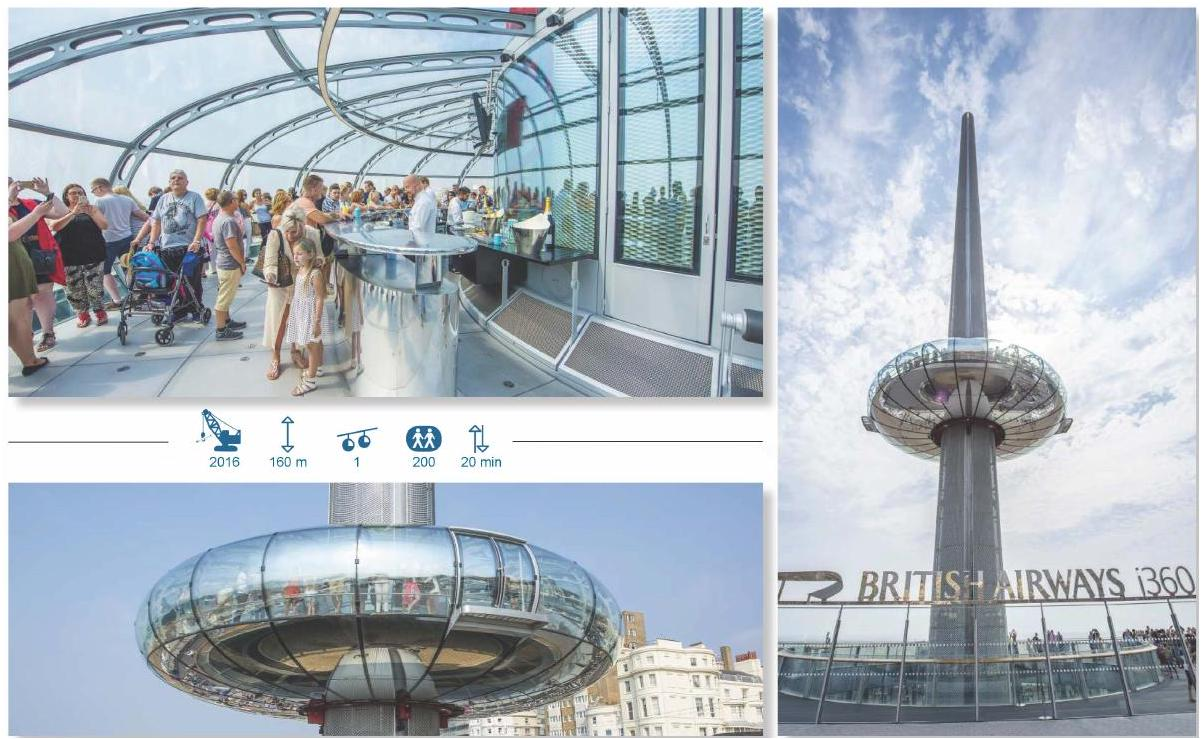
\includegraphics[alt={},max width=\textwidth]{cd8229cf-9637-40cc-9aaf-03c75c002f2c-01_739_1203_695_433}
\captionsetup{labelformat=empty}
\caption{Figure 1 - Vues de la tour British Airways i360}
\end{center}
\end{figure}

Conçue par les architectes Marks \& Barfield et réalisée en collaboration avec l'entreprise française POMA, la tour British Airways i360 (Figure 1) est une tour d'observation ascensionnelle installée à Brighton en Angleterre. La nacelle en forme de tore, dans laquelle embarquent jusqu'à 200 passagers, est uniquement animée d'un mouvement de translation verticale par rapport au mât encastré au sol. Cette nacelle, recouverte de verre, permet aux passagers de profiter d'une vue panoramique à 360° sur la ville balnéaire de Brighton, à une hauteur de 130 m au-dessus du niveau du sol. À ce titre, la tour British Airways i360 établit le record de l'ouvrage le plus élancé au monde grâce à son mât d'environ 160 m de haut et de 4 m de diamètre.

La tour s'inscrit dans une démarche de fonctionnement écologique visant à limiter sa consommation d'énergie. Seule l'énergie électrique consommée par le dispositif servant à mettre en mouvement la nacelle est étudiée dans ce sujet.

Le cahier des charges partiel du commanditaire de la tour British Airways i360 est décrit dans le Tableau 1.

\begin{table}[h]
\begin{center}
\begin{tabular}[t]{|l|l|}
\hline
Exigences & Descriptif \\
\hline
Id 1 - Accueillir les visiteurs & 4000 visiteurs chaque jour doivent pouvoir bénéficier de la vue panoramique \\
\hline
Id 2 - Proposer une visite en toute sécurité et dans le confort & Les accélérations et vitesses linéaires de la nacelle doivent être limitées quel que soit le nombre de passagers dans la nacelle \\
\hline
Id 3 - Limiter la consommation d'énergie électrique & La récupération d'énergie électrique à la descente doit être supérieure à la moitié de l'énergie électrique consommée à la montée \\
\hline
\end{tabular}
\captionsetup{labelformat=empty}
\caption{Tableau 1 - Cahier des charges partiel du commanditaire de la tour British Airways i360}
\end{center}
\end{table}

Certaines données et structures de l'ouvrage ont fait l'objet de modifications par rapport à la réalité pour des raisons de protection industrielle notamment.

\footnotetext{Objectifs de l'étude\\
Déterminer une loi de commande permettant de satisfaire les exigences de sécurité et de confort des passagers tout en optimisant la consommation d'énergie.
}Pour atteindre les objectifs fixés, la démarche retenue dans le sujet est la suivante :

\begin{itemize}
  \item[-] décrire le mouvement souhaité de la nacelle conformément aux exigences du commanditaire ;
  \item[-] établir les modèles cinématique et dynamique du dispositif servant à mettre en mouvement la nacelle;
  \item[-] synthétiser une loi de commande de l'actionneur mettant en mouvement la nacelle conformément aux exigences du commanditaire;
  \item[-] vérifier la performance liée à la consommation d'énergie électrique de l'actionneur.
\end{itemize}

\section*{Partie A - Étude du mouvement souhaité de la nacelle}
Objectif\\
Décrire le mouvement souhaité de la nacelle conforme à la visite panoramique, aux exigences de sécurité et de confort des passagers.

\section*{I - Modélisation du mouvement souhaité de la nacelle}
Notations

\begin{itemize}
  \item[-] le sol avec le mât, de repère associé $\mathcal{R}_{0}=\left(O_{0}, \vec{x}, \vec{y}, \vec{z}\right)$, supposé galiléen dans tout le sujet, est repéré par le chiffre 0 ;
  \item[-] la nacelle est repérée par la lettre $N$. Son centre de gravité $G$ est supposé porté par l'axe $\left(O_{0}, \vec{z}\right)$ au cours du mouvement de la nacelle ;
  \item[-] la position linéaire souhaitée de la nacelle $N$ par rapport au sol 0 est notée $\overrightarrow{O_{0} G}=z_{s}(t) \cdot \vec{z}$ exprimée en m;
  \item[-] la vitesse linéaire souhaitée du centre de gravité $G$ de la nacelle $N$ par rapport au sol 0 est notée $\vec{V}_{G, N / 0}=v_{s}(t) \cdot \vec{z}$ exprimée en $\mathrm{m} \cdot \mathrm{s}^{-1}$;
  \item[-] l'accélération linéaire souhaitée du centre de gravité $G$ de la nacelle $N$ par rapport au sol 0 est notée $\vec{a}_{G, N / 0}=$ $a_{s}(t) \cdot \vec{z}$ exprimée en $\mathrm{m} \cdot \mathrm{s}^{-2}$.
\end{itemize}

Le cycle souhaité de la nacelle suit les étapes suivantes :

\begin{itemize}
  \item[-] une phase ascensionnelle de la nacelle, d'une durée maximale de 6 minutes, décomposée en sous-phases dont la description est fournie ci-dessous,
  \begin{itemize}
    \item[-] les passagers ont fini d'embarquer dans la nacelle immobile à l'instant $t=t_{0}=0$, au niveau du sol $\left(z_{s}\left(t_{0}\right)=0\right.$ et $v_{s}\left(t_{0}\right)=0$ ), appelé niveau inférieur ;
    \item[-] le début de l'ascension s'effectue à accélération linéaire constante, notée $a_{1}>0$, et dure $t_{1}$ secondes. La vitesse linéaire atteinte à l'instant $t_{1}$ est notée $v_{\text {nom }}$ et vaut $0,5 \mathrm{~m} \cdot \mathrm{~s}^{-1}$;
    \item[-] jusqu'à l'instant $t_{2}$, la vitesse est constante et égale à $v_{\text {nom }}$;
    \item[-] la fin de l'ascension, réalisée à accélération linéaire constante égale à $-a_{1}$, dure jusqu'à l'instant $t_{3}$;
  \end{itemize}
  \item[-] la nacelle est immobile au sommet de la tour, à une altitude souhaitée $z_{s}\left(t_{3}\right)=130 \mathrm{~m}$, appelé niveau supérieur. Les passagers restent dans la nacelle et peuvent observer la vue panoramique de la ville de Brighton et ses environs, pendant 10 minutes;
  \item[-] une phase descensionnelle de la nacelle, d'une durée maximale de 6 minutes, qui suit le même cycle que le cycle ascensionnel, mais avec des vitesses linéaires et accélérations linéaires souhaitées de signes opposés à la phase ascensionnelle. Les instants sont notés chronologiquement $t_{4}, t_{5}, t_{6}$ et $t_{7}$, avec $z_{s}\left(t_{4}\right)=130 \mathrm{~m}$ et $z_{s}\left(t_{7}\right)=0 \mathrm{~m}$.
\end{itemize}

Compte-tenu des règles de sécurité, des conditions d'accessibilité à la nacelle et afin d'assurer un confort optimal des passagers de la tour British Airways i360 durant leur visite et leur découverte de la ville de Brighton, les exigences retenues sont décrites dans le Tableau 2.

\begin{table}[h]
\begin{center}
\begin{tabular}[t]{|l|l|l|}
\hline
Exigences & Critères & Niveaux \\
\hline
Sécurité & Vitesse linéaire maximale de la nacelle & $v_{\text {max }}=0,6 \mathrm{~m} \cdot \mathrm{~s}^{-1}$ \\
\hline
Accessibilité & Précision de la position de la nacelle au niveau inférieur & $\Delta z \leqslant 5 \mathrm{~mm}$ \\
\hline
Panorama & Précision de la position de la nacelle au niveau supérieur & $\Delta z=\leqslant 5 \mathrm{~mm}$ \\
\hline
Confort & Accélération linéaire maximale de la nacelle & $a_{\text {max }}=0,015 \mathrm{~m} \cdot \mathrm{~s}^{-2}$ \\
\hline
\end{tabular}
\captionsetup{labelformat=empty}
\caption{Tableau 2 - Exigences relatives à la sécurité, à l'accessibilité, au panorama et au confort des passagers - Id 2}
\end{center}
\end{table}

Les évolutions temporelles de l'accélération linéaire souhaitée $a_{s}(t)$ et de la vitesse linéaire souhaitée $v_{s}(t)$ de la nacelle sont représentées sur la Figure 2.

\begin{figure}[h]
\begin{center}
  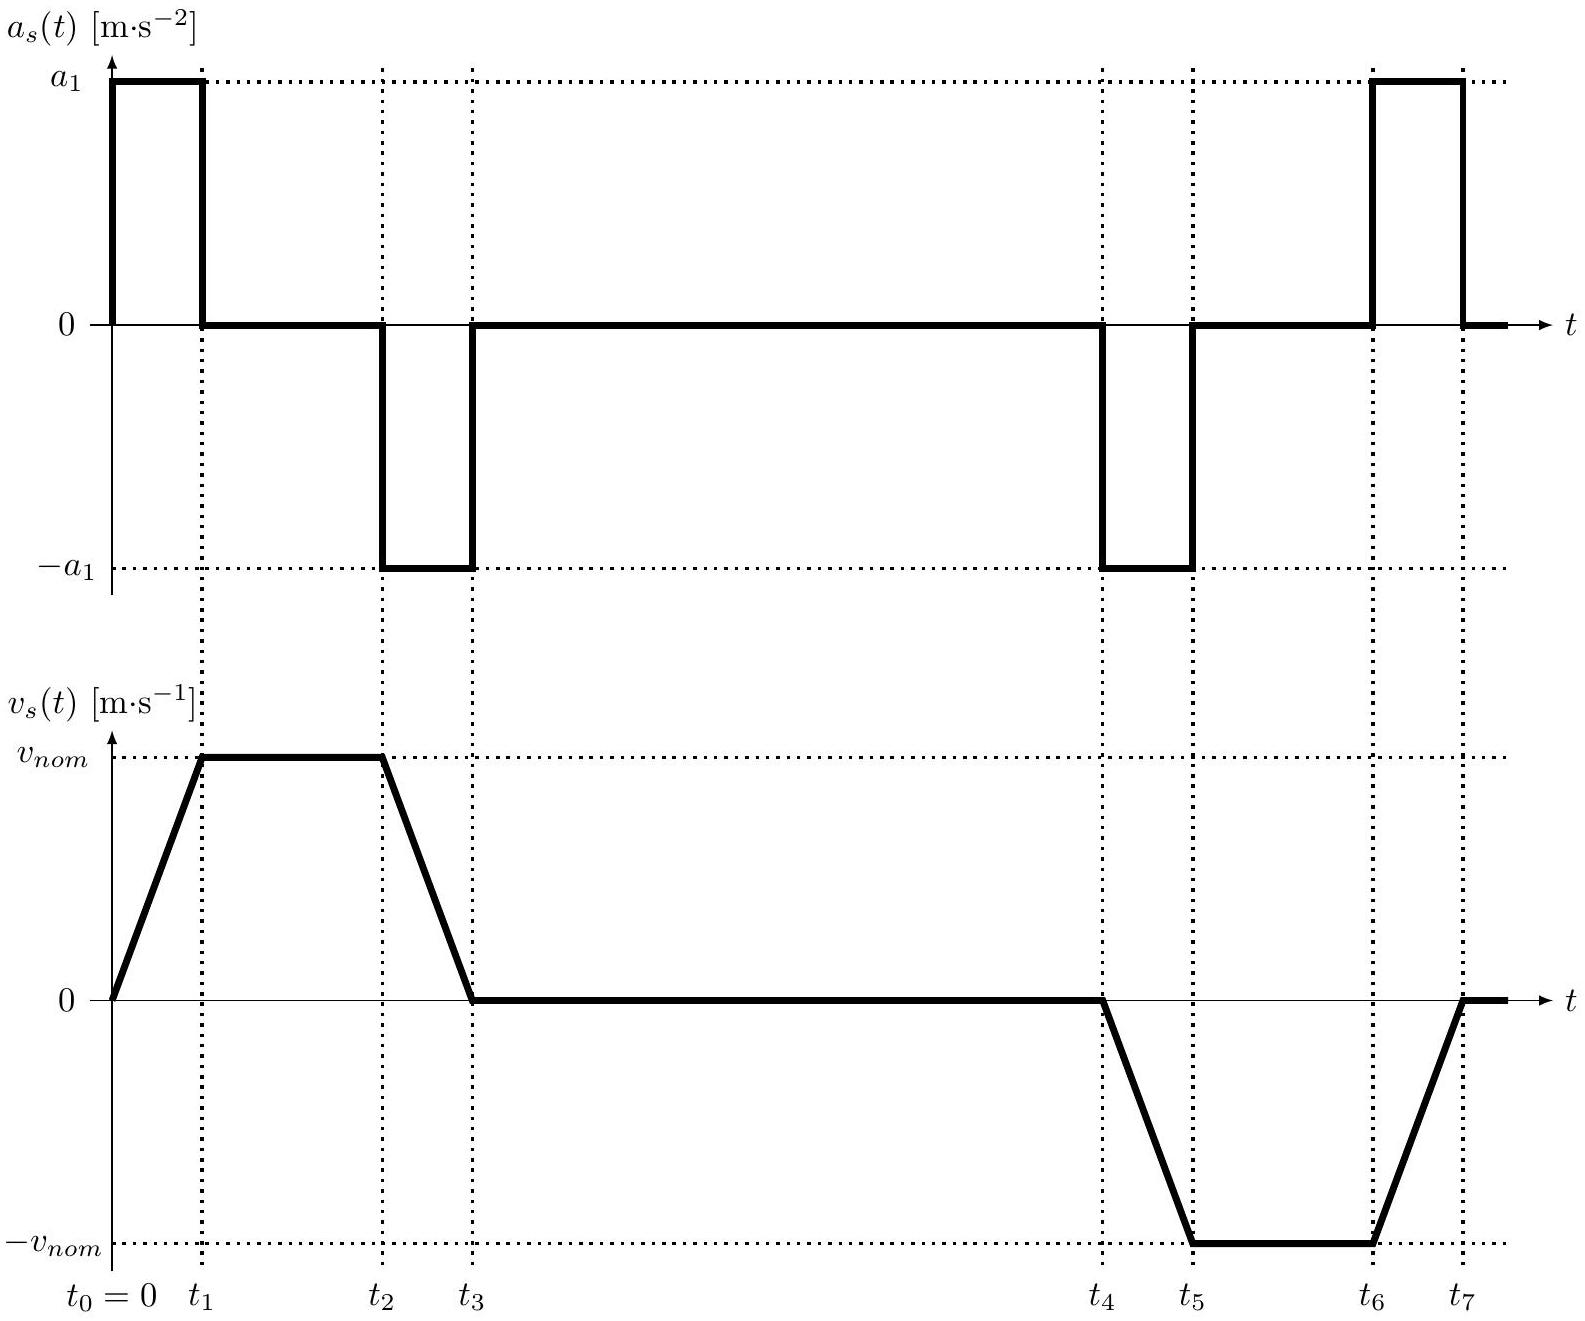
\includegraphics[alt={},max width=\textwidth]{cd8229cf-9637-40cc-9aaf-03c75c002f2c-03_1321_1585_130_243}
\captionsetup{labelformat=empty}
\caption{Figure 2 - Évolutions de l'accélération linéaire souhaitée $a_{s}(t)$ et de la vitesse linéaire souhaitée $v_{s}(t)$ de la nacelle $N$ sur un cycle complet}
\end{center}
\end{figure}

\begin{itemize}
  \item[Q1.] Sur la copie, et pour le cycle souhaité de la nacelle, tracer l'allure de l'évolution temporelle de la position linéaire souhaitée $z_{s}(t)$ de la nacelle $N$. Préciser les ordonnées caractéristiques $z_{s}\left(t_{3}\right)$ et $z_{s}\left(t_{7}\right)$.
  \item[Q2.] Vérifier que, si $t_{1}=40 \mathrm{~s}, t_{3}-t_{2}=40 \mathrm{~s}$ et $v_{\text {nom }}=0,5 \mathrm{~m} \cdot \mathrm{~s}^{-1}$, il est possible d'atteindre une altitude de 130 m en une durée $t_{3}$ maximale de 6 minutes. Par ailleurs, vérifier le respect de l'exigence de confort du Tableau 2.
\end{itemize}

Afin de respecter les exigences de sécurité et de confort des passagers, le profil de vitesse établi dans cette partie sera la consigne de vitesse linéaire. Toutefois, un suivi particulier de la position de la nacelle sera nécessaire pour atteindre les niveaux inférieur et supérieur avec précision (critères d'accessibilité et de panorama du Tableau 2).

\section*{II - Présentation de la cinématique de mise en mouvement de la nacelle}
L'élancement de l'ouvrage, la variation d'altitude nécessaire de la nacelle et le faible espace disponible dans le mât, ont conduit les ingénieurs à faire un choix de mise en mouvement de la nacelle par 2 types de câbles, dits tracteur et d'équilibrage, associés à un contrepoids (Figure 3).\\
La mise en mouvement de translation verticale de la nacelle $N$ de direction $\vec{z}$ par rapport au sol 0 (Figure 3) est réalisée par :

\begin{itemize}
  \item[-] 4 câbles d'équilibrage qui connectent la nacelle au contrepoids. Placés dans des rainures verticales situées à l'extérieur du mât, aux quatre points cardinaux, ces câbles assurent la stabilité horizontale de la nacelle. Chacun d'eux s'enroule autour d'une poulie d'équilibrage positionnée dans la partie supérieure du mât, puis redescend à l'intérieur du mât pour être fixé à son autre extrémité au contrepoids;
  \item[-] 1 câble tracteur, dont une de ses extrémités est fixée au sol (voir Ancrage au sol sur la Figure 3), s'enroule ou se déroule sur un tambour déporté du mât par l'intermédiaire de la poulie de renvoi. Le tambour est mis en rotation par un actionneur associé à un réducteur de vitesse.
\end{itemize}

\begin{figure}[h]
\begin{center}
  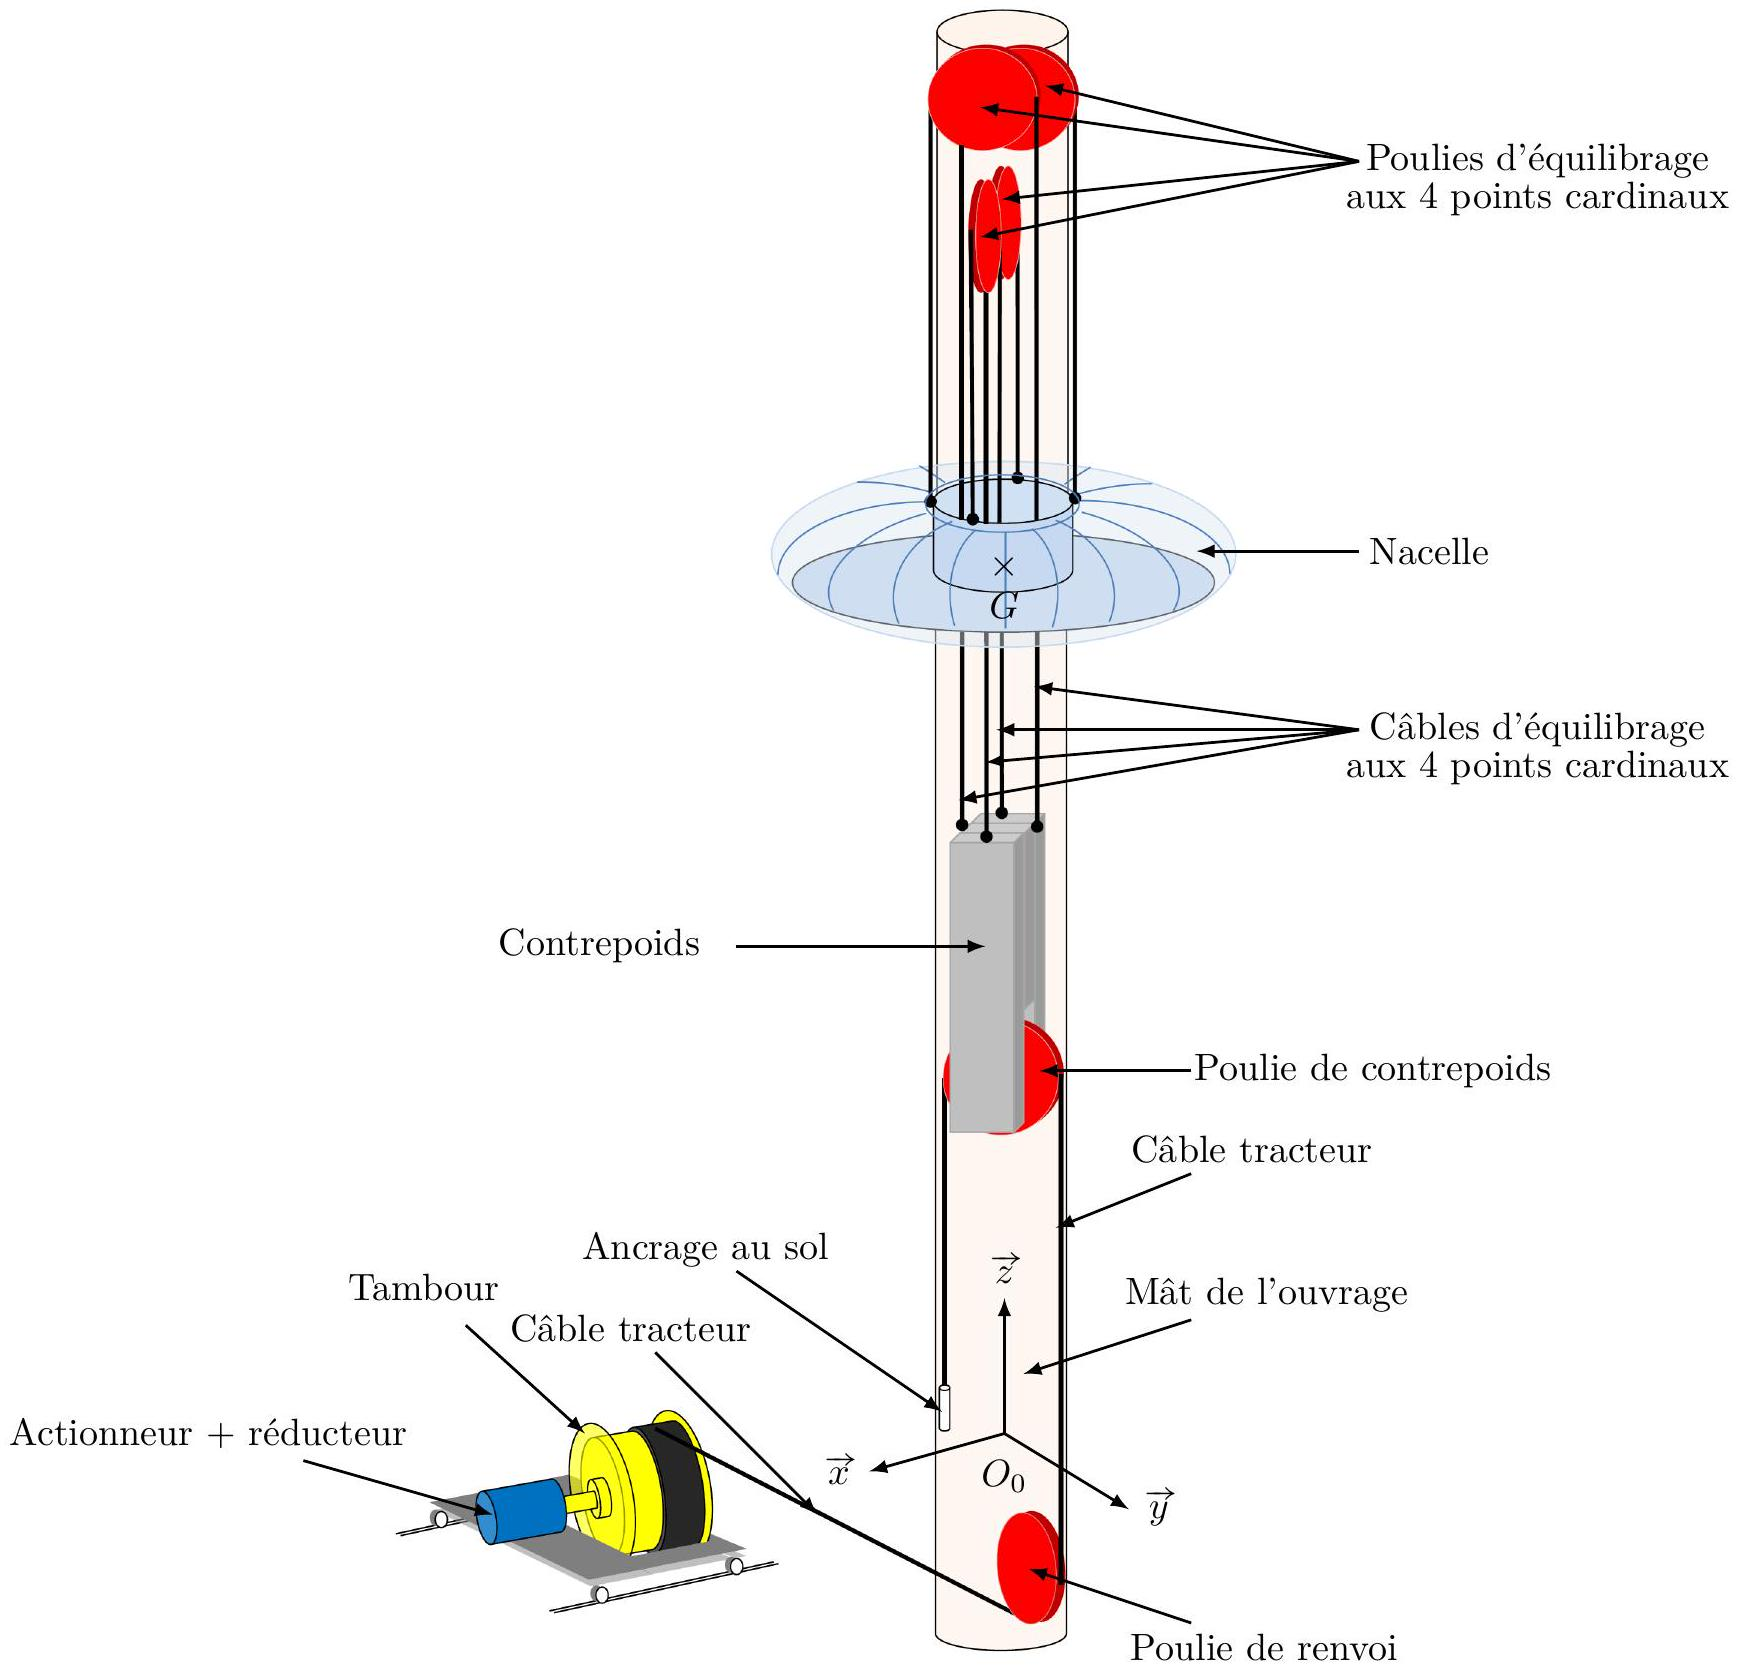
\includegraphics[alt={},max width=\textwidth]{cd8229cf-9637-40cc-9aaf-03c75c002f2c-04_1669_1739_130_164}
\captionsetup{labelformat=empty}
\caption{Figure 3 - Schéma technique de la tour British Airways i360}
\end{center}
\end{figure}

La structure de commande retenue pour la mise en mouvement de la nacelle $N$ de la tour British Airways i360 est proposée sur la Figure 4.\\
La grandeur $\omega_{m c}(t)$ représente la vitesse angulaire de consigne de l'actionneur. Elle est générée à partir de la loi d'évolution de la vitesse linéaire souhaitée $v_{s}(t)$ de la nacelle.\\
La grandeur $c_{\text {ref }}(t)$ est la grandeur de commande de l'ensemble \{Préactionneur + actionneur\}. Cet actionneur délivre au réducteur de vitesse une action mécanique du type couple, notée $c_{e m}(t)$.\\
Les grandeurs géométriques et cinématiques, notées $\theta_{m}(t)$ et $\omega_{m}(t)$ sont mesurées par des capteurs respectivement de position angulaire et de vitesse angulaire, situés au niveau de l'axe de rotation l'actionneur.\\
Afin de valider les exigences du cahier des charges du commanditaire Tableau 1, il est nécessaire d'établir un modèle global de la tour British Airways i360. Les parties B, C et D sont consacrées à l'élaboration de ce modèle et la partie E est consacrée à l'étude de la consommation d'énergie électrique du dispositif de mise en mouvement de la nacelle.

\begin{figure}[h]
\begin{center}
  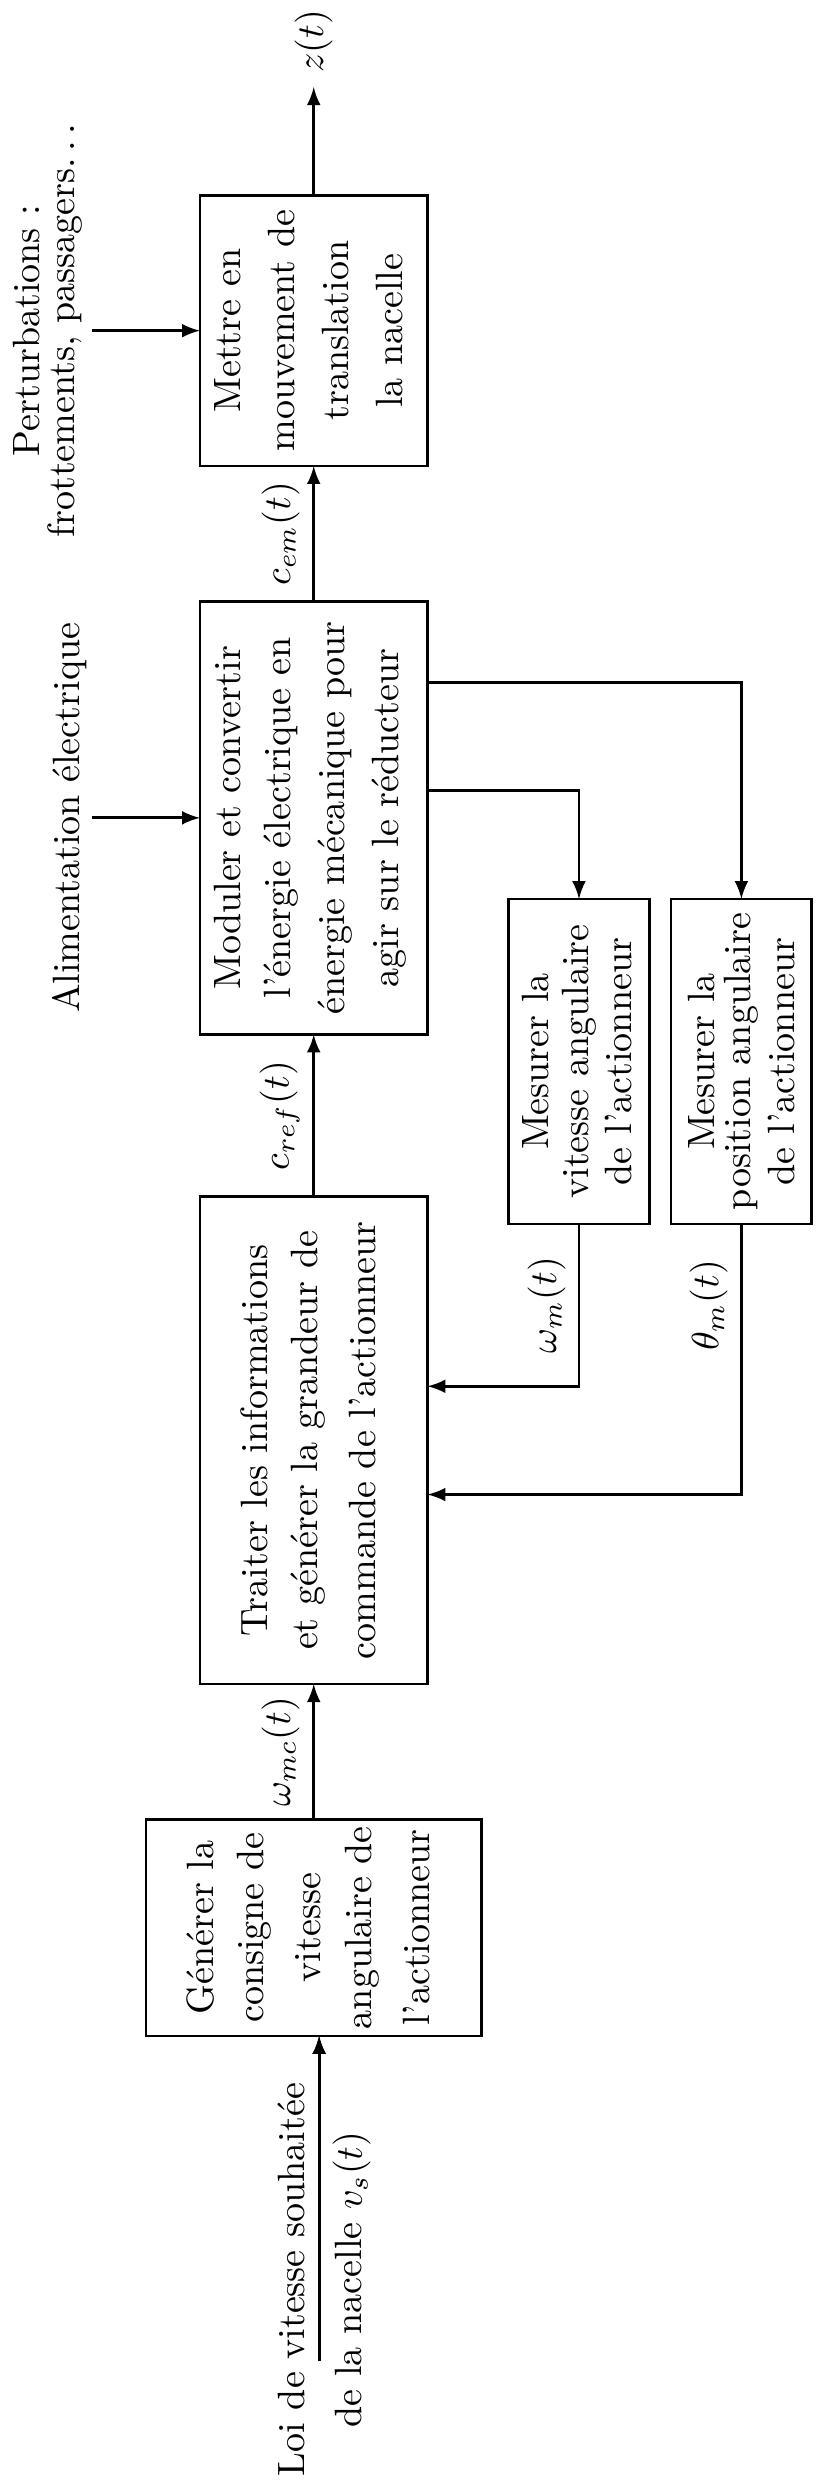
\includegraphics[alt={},max width=\textwidth]{cd8229cf-9637-40cc-9aaf-03c75c002f2c-05_2484_819_184_616}
\captionsetup{labelformat=empty}
\caption{Figure 4 - Structure fonctionnelle de la commande de l'actionneur pour la mise en mouvement de la nacelle}
\end{center}
\end{figure}

\section*{Partie B - Modélisation du mécanisme de transmission du mouvement}
Objectifs\\
Déterminer la loi entrée-sortie cinématique liant la vitesse angulaire $\omega_{m}(t)$ de l'actionneur à la vitesse de translation $v(t)$ du centre de gravité de la nacelle et vérifier que l'actionneur est en capacité de satisfaire le critère de vitesse linéaire de la nacelle.

Dans la suite du sujet, les 4 câbles d'équilibrage et les 4 poulies d'équilibrage seront respectivement modélisés par un seul câble d'équilibrage équivalent, noté ceq, et une seule poulie d'équilibrage équivalente, notée peq (Figure 5).

\begin{figure}[h]
\begin{center}
  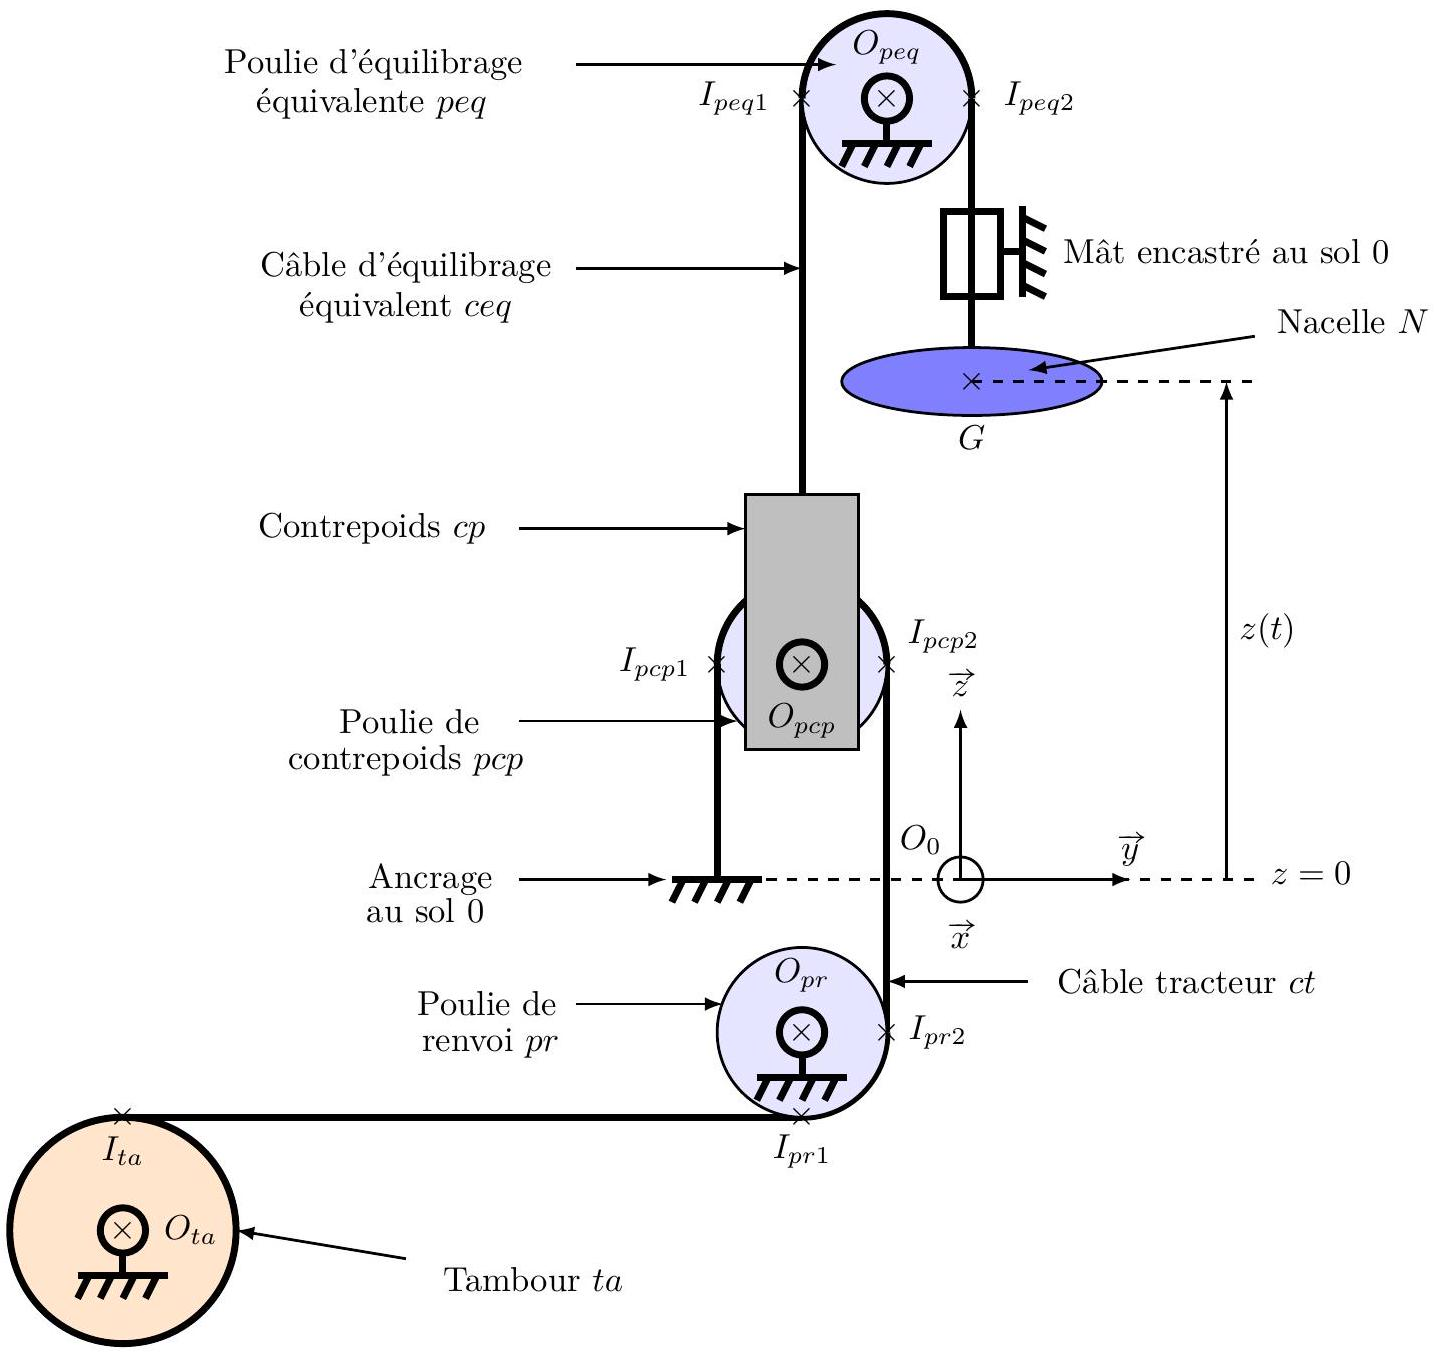
\includegraphics[alt={},max width=\textwidth]{cd8229cf-9637-40cc-9aaf-03c75c002f2c-06_1352_1436_625_310}
\captionsetup{labelformat=empty}
\caption{Figure 5 - Modélisation équivalente et paramétrage du mécanisme de mise en mouvement de la nacelle - Actionneur et réducteur non représentés}
\end{center}
\end{figure}

Notations

\begin{itemize}
  \item[-] le repère $\mathcal{R}_{0}=\left(O_{0}, \vec{x}, \vec{y}, \vec{z}\right)$ est lié au sol 0;
  \item[-] le centre de gravité de la nacelle $N$ est noté $G$ tel que $\overrightarrow{O_{0} G}=z(t) \cdot \vec{z}$;
  \item[-] la vitesse linéaire réelle du centre de gravité $G$ de la nacelle $N$ par rapport au sol 0 est notée $\vec{V}_{G, N / 0}=v(t) \cdot \vec{z}$;
  \item[-] le câble tracteur est noté $c t$ et le câble d'équilibrage équivalent est noté $c e q$;
  \item[-] le tambour, noté $t a$, de rayon $R_{t a}=1,5 \mathrm{~m}$, est en liaison pivot d'axe $\left(O_{t a}, \vec{x}\right)$ avec le sol 0 ;
  \item[-] la poulie de renvoi, notée $p r$, de rayon $R_{p r}$, est en liaison pivot d'axe $\left(O_{p r}, \vec{x}\right)$ avec le sol 0 ;
  \item[-] l'une des extrémités du câble d'équilibrage équivalent $c e q$ est fixée au contrepoids $c p$. La poulie de contrepoids, notée $p c p$, de rayon $R_{p c p}$, est en liaison pivot d'axe $\left(O_{p c p}, \vec{x}\right)$ avec le contrepoids $c p$;
  \item[-] la vitesse angulaire de la poulie de contrepoids $p c p$ par rapport au sol 0 est notée $\vec{\Omega}_{p c p / 0}=\omega_{p c p}(t) \cdot \vec{x}$;
\end{itemize}

\begin{itemize}
  \item[-] la vitesse angulaire du rotor de l'actionneur par rapport au sol 0 est notée $\vec{\Omega}_{m / 0}=\omega_{m}(t) \cdot \vec{x}$;
  \item[-] la vitesse angulaire du tambour $t a$ par rapport au sol 0 est notée $\vec{\Omega}_{t a / 0}=\omega_{t a}(t) \cdot \vec{x}$;
  \item[-] le réducteur de vitesse situé entre l'actionneur et le tambour possède un rapport de transmission $k_{\text {red }}=\frac{\omega_{t a}(t)}{\omega_{m}(t)}$ avec $k_{\text {red }}=1 / 153$;
  \item[-] la poulie d'équilibrage équivalente, notée $p e q$, de rayon $R_{p e q}$, est en liaison pivot d'axe $\left(O_{p e q}, \vec{x}\right)$ avec le sol 0. Sa vitesse angulaire par rapport au sol 0 est notée $\vec{\Omega}_{p e q / 0}=\omega_{p e q}(t) \cdot \vec{x}$;
  \item[-] les points $I_{t a}, I_{p r 1}, I_{p r 2}, I_{p c p 1}, I_{p c p 2}, I_{p e q 1}$ et $I_{p e q 2}$ sont les points géométriques délimitant les zones de contact entre les câbles et le tambour ou les poulies.
\end{itemize}

Hypothèses

\begin{itemize}
  \item[-] les câbles sont supposés inextensibles et sont constamment tendus ;
  \item[-] les diamètres des câbles sont négligés par rapport aux dimensions des poulies et du tambour ;
  \item[-] les contacts entre le câble tracteur $c t$ et la poulie de renvoi $p r$, entre le câble tracteur $c t$ et la poulie de contrepoids $p c p$ ainsi qu'entre le câble d'équilibrage équivalent $c e q$ et la poulie d'équilibrage équivalent peq sont supposés sans glissement relatif.
\end{itemize}

Les concepteurs ont fait le choix d'enrouler le câble tracteur $c t$ en une seule couche sur le tambour d'enroulement ta afin d'éviter notamment les problèmes de glissement du câble tracteur sur lui-même et de bénéficier d'un diamètre d'enroulement constant. Un dispositif spécifique non étudié dans le sujet permet de garantir une répartition convenable du câble tracteur $c t$ sur le tambour $t a$ en une seule couche.

L'étude porte dans un premier temps sur la partie de la chaîne cinématique située entre le rotor de l'actionneur et la poulie de contrepoids (Figure 5).

Q3. En considérant le non-glissement du câble tracteur $c t$ par rapport au tambour ta, calculer la vitesse $\vec{V}_{I_{t a}, c t / 0}$ en fonction de $R_{t a}, k_{\text {red }}$ et $\omega_{m}(t)$.

Q4. Quelle(s) hypothèse(s) permet(tent) de justifier que $\vec{V}_{I_{t a}, c t / 0} \cdot \vec{y}=\vec{V}_{I_{p c p 2}, c t / 0} \cdot \vec{z}$ ?\\
Q5. En supposant le non-glissement entre le câble tracteur $c t$ et la poulie de contrepoids $p c p$, déterminer la relation entre $\vec{V}_{I_{p c p 2}, p c p / 0}$ et $\omega_{m}(t), k_{\text {red }}$ et $R_{t a}$.\\
L'étude porte à présent sur le mécanisme composé du contrepoids $c p$ et de la poulie de contrepoids $p c p$. Sachant que l'une des extrémités du câble tracteur $c t$ est fixée au sol (voir Ancrage au sol sur la Figure 5) et que, par hypothèse, il y a non-glissement entre la poulie de contrepoids $p c p$ et le câble tracteur $c t$, alors $\vec{V}_{I_{p c p 1}, p c p / 0}=\overrightarrow{0}$.

Q6. Quelle relation lie $\vec{V}_{O_{p c p}, p c p / 0}$ et $\vec{V}_{O_{p c p}, c e q / 0}$ ? Justifier votre réponse.\\
Q7. Exprimer $\vec{V}_{O_{p c p}, c e q / 0}$ en fonction de $\vec{V}_{I_{p c p 2}, p c p / 0}$, puis en fonction de $\omega_{m}(t)$ et des données géométriques utiles.\\
Pour finir, la relation recherchée s'obtient en effectuant l'étude du mécanisme composé du câble d'équilibrage équivalent ceq, de la poulie d'équilibrage équivalente peq et de la nacelle $N$.

Q8. Déterminer la relation liant $\vec{V}_{O p c p, c e q / 0}$ et $\vec{V}_{G, N / 0}$. Présenter clairement la démarche mise en œuvre.\\
Q9. En déduire que la relation liant $v(t)$ et $\omega_{m}(t)$ s'écrit sous la forme $v(t)=k_{\text {cin }} \cdot \omega_{m}(t)$. Préciser l'expression de $k_{c i n}$ en fonction de $k_{\text {red }}$ et $R_{t a}$.

L'actionneur utilisé sur l'ouvrage possède une vitesse de rotation nominale $\omega_{m_{n o m}}$ de $980 \mathrm{tr} \cdot \mathrm{min}^{-1}$.\\
Q10. Conclure quant à la capacité de l'actionneur à satisfaire le critère de vitesse nominale $v_{\text {nom }}=0,5 \mathrm{~m} \cdot \mathrm{~s}^{-1}$ de la nacelle $N$.

La loi entrée-sortie cinématique du mécanisme permettant la mise en mouvement de la nacelle par rapport au sol est maintenant mise en place. Dans l'objectif de s'assurer du respect de l'exigence Id 2 relative à la sécurité, à l'accessibilité et au panorama et au confort des passagers, il est nécessaire de déterminer l'équation de mouvement de la nacelle $N$.

\section*{Partie C - Modélisation de la dynamique de la nacelle}
Objectif\\
Déterminer l'équation de mouvement de la nacelle $N$ par rapport au sol 0 en fonction du couple électromagnétique $c_{e m}(t)$ développé par l'actionneur.

\section*{I - Présentation de la modélisation}
La modélisation retenue pour la détermination de l'équation de mouvement de la nacelle $N$ est fournie sur la Figure 5. Les caractéristiques géométriques, massiques et inertielles des solides sont fournies dans le Tableau 3.

\begin{table}[h]
\begin{center}
\begin{tabular}[t]{|l|l|}
\hline
Solides & Caractéristiques \\
\hline
Sol 0 et mât & Référentiel $\mathcal{R}_{0}=\left(O_{0}, \vec{x}, \vec{y}, \vec{z}\right)$ supposé galiléen \\
\hline
Rotor de l'actionneur $m$ et du réducteur & Moment d'inertie de l'ensemble rapporté à l'axe de rotation de l'actionneur $J_{m r}=11 \mathrm{~kg} \cdot \mathrm{~m}^{2}$ \\
\hline
Tambour $t a$ & Moment d'inertie autour de l'axe $\left(O_{t a}, \vec{x}\right) J_{t a}=24120 \mathrm{~kg} \cdot \mathrm{~m}^{2}$ \\
\hline
Poulie de renvoi $p r$ & Poids et inertie négligés \\
\hline
Contrepoids $c p$ & Centre de gravité $O_{p c p}$ et masse $M_{c p}=72000 \mathrm{~kg}$ \\
\hline
Poulie de contrepoids $p c p$ & Poids et inertie négligés \\
\hline
Poulie d'équilibrage équivalente peq & Moment d'inertie autour de l'axe $\left(O_{p e q}, \vec{x}\right) J_{p e q}=20300 \mathrm{~kg} \cdot \mathrm{~m}^{2}$ \\
\hline
$N_{p}=$ Nacelle $N$ avec $n=200$ passagers & Centre de gravité $G$ et masse $M_{N p}=110000 \mathrm{~kg}$ (passagers inclus) \\
\hline
Passagers & Masse $m_{p}=80 \times n$. Masse maximale de 16000 kg \\
\hline
Câbles tracteur $c t$ et équivalent $c e q$ & Poids négligés \\
\hline
\end{tabular}
\captionsetup{labelformat=empty}
\caption{Tableau 3 - Caractéristiques géométriques, massiques et inertielles des solides}
\end{center}
\end{table}

Notations

\begin{itemize}
  \item[-] l'action mécanique du solide $S_{i}$ sur le solide $S_{j}$, exprimée au point $P$ dans la base $b=(\vec{x}, \vec{y}, \vec{z})$, est notée $\left\{\mathcal{T}_{S_{i} \rightarrow S_{j}}\right\}=\left\{\begin{array}{c}X_{i j} \cdot \vec{x}+Y_{i j} \cdot \vec{y}+Z_{i j} \cdot \vec{z} \\ L_{i j} \cdot \vec{x}+M_{i j} \cdot \vec{y}+N_{i j} \cdot \vec{z}\end{array}\right\}_{P} ;$
  \item[-] la puissance galiléenne de l'action mécanique du solide $S_{i}$ sur le solide $S_{j}$ est notée $P_{S_{i} \rightarrow S_{j} / 0}$;
  \item[-] la puissance des inter-efforts entre les solides $S_{i}$ et $S_{j}$ est notée $P_{S_{i} \leftrightarrow S_{j}}$;
  \item[-] l'action de la pesanteur agissant sur un solide de masse $M$ est modélisée par un torseur glisseur, en son centre de gravité et de résultante $-M \cdot g \cdot \vec{z}$ avec $g=9,81 \mathrm{~m} \cdot \mathrm{~s}^{-2}$;
  \item[-] l'action mécanique du stator de l'actionneur sur le rotor est modélisée par un torseur couple de moment noté $c_{e m}(t) \cdot \vec{x}$;
  \item[-] la vitesse linéaire du contrepoids $v_{c p}(t)$ par rapport au sol est définie par $v_{c p}(t)=\frac{\mathrm{d} \overrightarrow{O_{0} O_{p c p}} \cdot \vec{z}}{\mathrm{~d} t}$;
  \item[-] $\vec{V}_{I_{p c p 2}, c t / 0}=v_{c t}(t) \cdot \underset{\sim}{\vec{z}}$.
\end{itemize}

Relations cinématiques\\
Indépendamment des résultats précédents, les relations cinématiques suivantes sont adoptées :

\begin{itemize}
  \item[-] la vitesse linéaire $v(t)$ de la nacelle $N$ par rapport au sol 0 est liée à la vitesse angulaire $\omega_{m}(t)$ du rotor de l'actionneur par l'équation
$$
v(t)=k_{c i n} \cdot \omega_{m}(t)=\frac{1}{204} \cdot \omega_{m}(t) ;
$$
  \item[-] la vitesse linéaire $v_{c p}(t)$ du contrepoids $c p$ par rapport au sol 0 est liée à la vitesse linéaire $v(t)$ de la nacelle par l'équation
$$
v_{c p}(t)=-v(t) ;
$$
  \item[-] la vitesse linéaire $v_{c t}(t)$ du câble tracteur $c t$ par rapport au sol 0 est liée à la vitesse linéaire $v(t)$ de la nacelle par l'équation
$$
v_{c t}(t)=-2 \cdot v(t) ;
$$
  \item[-] la vitesse angulaire $\omega_{t a}(t)$ du tambour $t a$ par rapport au sol 0 est liée à la vitesse angulaire $\omega_{m}(t)$ du rotor par l'équation
$$
\omega_{t a}(t)=k_{r e d} \cdot \omega_{m}(t) ;
$$
  \item[-] la vitesse angulaire $\omega_{p e q}(t)$ de la poulie d'équilibrage équivalente $p e q$ par rapport au sol 0 est liée à la vitesse linéaire $v(t)$ de la nacelle $N$ par l'équation
$$
v(t)=R_{p e q} \cdot \omega_{p e q}(t) .
$$
\end{itemize}

Hypothèses

\begin{itemize}
  \item[-] toutes les liaisons sont supposées parfaites;
  \item[-] les forces aérodynamiques agissant sur la nacelle $N$ et les perturbations liées au vent sont négligées.
\end{itemize}

\section*{II - Détermination d'une équation de mouvement de la nacelle}
Soit $\Sigma$ l'ensemble composé de la nacelle $N$ avec $n=200$ passagers, du rotor de l'actionneur, du réducteur, du tambour ta, des différentes poulies, des câbles (tracteur $c t$ et d'équilibrage équivalent $c e q$ ) et du contrepoids $c p$. L'équation de mouvement de la nacelle $N$ va être déterminée par application du théorème de l'énergie cinétique à l'ensemble $\Sigma$.

Q11. Déterminer les expressions des énergies cinétiques, par rapport au référentiel galiléen $\mathcal{R}_{0}$, en fonction des caractéristiques massiques et inertielles :

\begin{itemize}
  \item[-] du sous-ensemble $N_{p}=\{$ nacelle $N+200$ passagers $\}$, notée $E_{c, N p / 0}$, en fonction de $v(t)$;
  \item[-] du sous-ensemble \{rotor de l'actionneur + réducteur\}, notée $E_{c, m r / 0}$, en fonction de $\omega_{m}(t)$;
  \item[-] du tambour $t a$, notée $E_{c, t a / 0}$, en fonction de $\omega_{t a}(t)$.
\end{itemize}

Q12. Déterminer l'ensemble des énergies cinétiques des autres solides qui composent l'ensemble $\Sigma$ par rapport à $\mathcal{R}_{0}$ en fonction de leurs vitesses respectives par rapport au sol 0.

Q13. Montrer que l'énergie cinétique de l'ensemble $\Sigma$ en mouvement par rapport au sol 0 peut s'écrire sous la forme

$$
E_{c, \Sigma / 0}=\frac{1}{2} \cdot J_{e q_{\Sigma}} \cdot \omega_{m}^{2}(t)
$$

où l'expression de $J_{e q_{\Sigma}}$ est à préciser en fonction de $M_{N p}, M_{c p}, J_{m r}, J_{t a}, J_{\text {peq }}, R_{\text {peq }}, k_{\text {red }}$ et $k_{\text {cin }}$.\\
Q14. Sachant que $J_{e q_{\Sigma}}=16,8 \mathrm{~kg} \cdot \mathrm{~m}^{2}$ (pour $n=200$ passagers), montrer que la variation relative de $J_{e q_{\Sigma}}$ due à l'absence des passagers $(n=0)$ dans la nacelle $N$, est négligeable.

Q15. Déterminer les puissances galiléennes des actions mécaniques de la pesanteur sur le sous-ensemble $N_{p}=\{$ nacelle $N+200$ passagers\} notée $P_{p e s \rightarrow N p / 0}$ et sur le contrepoids $c p$ notée $P_{p e s \rightarrow c p / 0}$, notamment en fonction de $v(t)$.

Q16. Après avoir listé toutes les puissances des actions mécaniques extérieures agissant sur l'ensemble $\Sigma$ (sauf celles déterminées Q15), déterminer leurs expressions ou justifier quand elles sont nulles.

Q17. Quelle(s) hypothèse(s) permet(tent) de justifier que la puissance des actions mécaniques intérieures à l'ensemble isolé $\Sigma$ est nulle?

Q18. Par application du théorème de l'énergie cinétique à l'ensemble isolé $\Sigma$, montrer que, dans le cadre des hypothèses formulées, l'équation de mouvement de la nacelle $N$ s'écrit sous la forme

$$
J_{e q_{\Sigma}} \cdot \frac{\mathrm{d} \omega_{m}(t)}{\mathrm{d} t}=c_{e m}(t)-C_{0} .
$$

Eq. 1\\
Préciser l'expression de $C_{0}$.

\section*{III - Validation de l'équation de mouvement}
La puissance électromagnétique $p_{e m}(t)=c_{e m}(t) \cdot \omega_{m}(t)$ délivrée par l'actionneur a été mesurée lors d'essais réalisés sur la tour British Airways i360, avec une masse équivalente à celle de 200 passagers embarqués dans la nacelle. La Figure 6 présente l'évolution de cette puissance pendant les phases de fonctionnement à vitesse constante.\\
La validation de l'équation de mouvement de la nacelle est réalisée uniquement pendant les phases de fonctionnement à vitesse linéaire constante, entre les instants $t_{1}$ et $t_{2}$ puis $t_{5}$ et $t_{6}$, définis en Partie A-I.

Q19. Lors de la phase ascensionnelle de la nacelle à vitesse linéaire constante $v_{\text {nom }}$, simplifier l'équation de mouvement Eq. 1. En déduire l'expression de la puissance électromagnétique délivrée par l'actionneur $p_{e m}(t)$, en phase de vitesse constante de la nacelle. Exprimer le résultat en fonction de $C_{0}, v_{\text {nom }}$ et $k_{\text {cin }}$.

Q20. Comparer l'évolution de la puissance électromagnétique $p_{e m}(t)$ prévue par le modèle établi et celle mesurée in situ sur la tour British Airways i360 (Figure 6). Conclure sur la validité du modèle établi dans cette partie, et préciser quelle hypothèse (parmi celles formulées dans le Tableau 3) est à remettre en cause.

Une équation de mouvement de la nacelle $N$ par rapport au sol 0 plus représentative de la réalité s'écrit sous la forme

$$
J_{0} \cdot \frac{\mathrm{~d} \omega_{m}(t)}{\mathrm{d} t}=\Delta c_{e m}(t)-c_{R}(t)+k_{c r z} \cdot z(t) .
$$

Eq. 2

\begin{figure}[h]
\begin{center}
  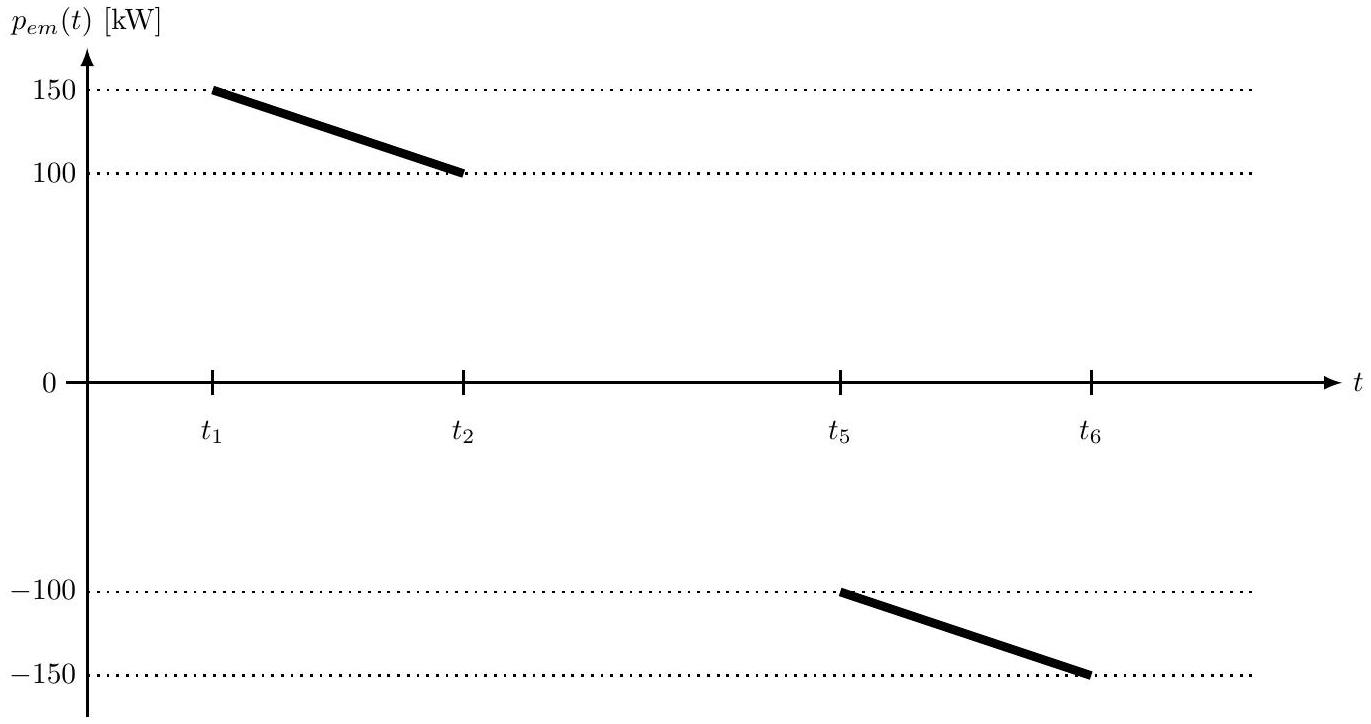
\includegraphics[alt={},max width=\textwidth]{cd8229cf-9637-40cc-9aaf-03c75c002f2c-10_724_1371_130_347}
\captionsetup{labelformat=empty}
\caption{Figure 6 - Évolution de la puissance électromagnétique fournie par l'actionneur pendant les phases à vitesse linéaire constante mesurée in situ sur la tour British Airways 360}
\end{center}
\end{figure}

Notations

\begin{itemize}
  \item[-] $J_{0}$ est le moment d'inertie équivalent à l'ensemble des solides en mouvement rapporté sur l'axe de rotation de l'actionneur ;
  \item[-] $\omega_{m}(t)$ représente la vitesse angulaire du rotor de l'actionneur, exprimée en $\mathrm{rad} \cdot \mathrm{s}^{-1} . \Omega_{m}(p)$ est sa transformée de Laplace ;
  \item[-] $\theta_{m}(t)$ représente la position angulaire du rotor de l'actionneur, exprimée en $\mathrm{rad} . \Theta_{m}(p)$ est sa transformée de Laplace ;
  \item[-] $z(t)=k_{\text {cin }} \cdot \theta_{m}(t)$ représente l'altitude de la nacelle $N$ par rapport au sol 0, exprimée en m. $Z(p)$ est sa transformée de Laplace ;
  \item[-] $\Delta c_{e m}(t)$ représente la variation de couple électromagnétique par rapport à la position de départ à l'instant $t=t_{0}=0$, exprimée en $\mathrm{N} \cdot \mathrm{m}$. Au niveau du sol $z\left(t_{0}\right)=0, \theta_{m}\left(t_{0}\right)=0, \omega_{m}\left(t_{0}\right)=0$ et $\Delta c_{e m}\left(t_{0}\right)=0 . \Delta C_{e m}(p)$ est sa transformée de Laplace ;
  \item[-] pour prendre en compte des perturbations en couple, dus notamment aux efforts de liaisons et la présence ou non de passagers dans la nacelle, le modèle est complété par le terme $c_{R}(t)$ exprimé en $\mathrm{N} \cdot \mathrm{m} . C_{R}(p)$ est sa transformée de Laplace ;
  \item[-] $k_{c r z}$ est un coefficient traduisant la dépendance entre l'action mécanique résistante rapportée sur l'axe de rotation du rotor de l'actionneur et l'altitude de la nacelle $z(t)$, avec $k_{c r z}>0$.
\end{itemize}

Q21. Déterminer la fonction de transfert $H_{1}(p)$ telle que $\Omega_{m}(p)=H_{1}(p) \cdot\left(\Delta C_{e m}(p)-C_{R}(p)\right)$ en considérant les conditions de Heaviside vérifiées. Justifier que cette fonction de transfert est caractéristique d'un modèle de système instable.

L'actionneur retenu pour la tour British Airways i360 fournit une puissance maximale de 200 kW, pour une vitesse de rotation nominale de $980 \mathrm{tr} \cdot \mathrm{min}^{-1}$. Compte-tenu des puissances mises en jeu, et afin de valider les exigences liées à la sécurité et au confort des visiteurs, il est nécessaire de stabiliser la commande de la nacelle et de maîtriser, par asservissement, les évolutions des grandeurs géométriques et cinématiques.

\section*{Partie D - Synthèse d'une loi de commande de l'actionneur}
Objectif\\
Proposer une loi de commande de l'actionneur mettant en mouvement la nacelle et vérifier les exigences relatives à la sécurité, à l'accessibilité, au panorama et au confort des passagers.

La partie précédente a montré l'instabilité d'une commande en couple de l'actionneur. Pour contrôler la vitesse de la nacelle $N$, il est nécessaire de stabiliser le comportement dynamique de l'ensemble $\Sigma$ régi par l'équation Eq. 2. L'actionneur, délivrant le couple $c_{e m}(t)$, est commandé en couple par l'intermédiaire du préactionneur par la grandeur $c_{\text {ref }}(t)$.

\section*{Rappels et notations}
\begin{itemize}
  \item[-] $\omega_{m c}(t)$ représente la vitesse angulaire de consigne du rotor de l'actionneur, exprimée en $\operatorname{rad} \cdot \mathrm{s}^{-1} . \Omega_{m c}(p)$ est sa transformée de Laplace ;
  \item[-] $\omega_{m}(t)$ représente la vitesse angulaire du rotor de l'actionneur, exprimée en $\mathrm{rad} \cdot \mathrm{s}^{-1} . \Omega_{m}(p)$ est sa transformée de Laplace;
  \item[-] $\theta_{m}(t)$ représente la position angulaire du rotor de l'actionneur, exprimée en $\operatorname{rad} . \Theta_{m}(p)$ est sa transformée de Laplace;
  \item[-] $c_{e m}(t)$ est l'action mécanique du type couple générée par l'actionneur sur le réducteur de vitesse exprimée en $\mathrm{N} \cdot \mathrm{m}$;
  \item[-] $c_{\text {ref }}(t)$ est la grandeur de commande de l'ensemble \{Préactionneur + actionneur\} exprimée en $\mathrm{N} \cdot \mathrm{m}$. Le temps de réponse de cet ensemble étant faible comparativement à la dynamique du système étudié, on considère $c_{e m}(t)=c_{r e f}(t)$ et $\Delta c_{e m}(t)=\Delta c_{\text {ref }}(t)$;
  \item[-] $c_{R}(t)$ représente une action mécanique résistante rapportée sur l'axe de rotation du rotor de l'actionneur, exprimée en $\mathrm{N} \cdot \mathrm{m} . C_{R}(p)$ est sa transformée de Laplace.
\end{itemize}

\section*{I - Stabilisation du comportement dynamique de l'ensemble de mise en mouvement de la nacelle}
Objectif\\
Élaborer une commande de l'actionneur assurant la stabilité de la dynamique de l'ensemble de mise en mouvement de la nacelle.

Pour contrôler la vitesse linéaire $v(t)$ de la nacelle $N$, il est nécessaire de stabiliser le comportement dynamique de l'ensemble $\Sigma$ régi par l'équation Eq.2. À cet effet, la variation de couple $\Delta c_{\text {ref }}(t)=\Delta c_{e m}(t)$ est commandée par un retour informationnel fonction de la vitesse angulaire de consigne et de la vitesse angulaire du rotor de l'actionneur telle que :

$$
\Delta c_{e m}(t)=-K_{1} \cdot \omega_{m}(t)-K_{2} \cdot \int_{0}^{t}\left(\omega_{m}(x)-K_{3} \cdot \omega_{m c}(x)\right) \cdot \mathrm{d} x \quad \text { Eq. } 3
$$

où $K_{1}, K_{2}$ et $K_{3}$ sont des constantes positives à déterminer.\\
Q22. À l'aide des équations Eq. 2, Eq. 3, en l'absence de perturbation $\left(C_{R}(p)=0\right)$ et en supposant les conditions de Heaviside vérifiées, déterminer l'expression de la fonction de transfert $H_{\text {stab }}(p)$ en fonction de $K_{1}, K_{2}, K_{3}$, $J_{0}, k_{c r z}$ et $k_{c i n}$ telle que :

$$
\Omega_{m}(p)=H_{s t a b}(p) \cdot \Omega_{m c}(p)
$$

Afin de limiter les oscillations des câbles et leurs sollicitations en traction notamment, le comportement souhaité de la boucle de stabilisation est telle que $H_{\text {stab }}(p)$ s'écrive sous la forme :

$$
H_{s t a b}(p)=\frac{1}{1+\frac{2 \xi_{s}}{\omega_{0 s}} \cdot p^{+} \frac{p^{2}}{\omega_{0 s}^{2}}} .
$$

Le cahier des charges relatif à la boucle de stabilisation est fourni dans le Tableau 4.

\begin{table}[h]
\begin{center}
\begin{tabular}[t]{|l|l|l|}
\hline
Performances & Critères & Niveaux \\
\hline
Stabilité & Facteur d'amortissement de la boucle de stabilisation & $\xi_{s} \geqslant 1$ \\
\hline
Rapidité & Pulsation propre du système non amorti de la boucle de stabilisation & $\omega_{0 s}=3 \mathrm{rad} \cdot \mathrm{s}^{-1}$ \\
\hline
\end{tabular}
\captionsetup{labelformat=empty}
\caption{Tableau 4 - Cahier des charges de la boucle de stabilisation}
\end{center}
\end{table}

Q23. Déterminer les expressions littérales de $K_{1}, K_{2}$ et $K_{3}$ en fonction de $\xi_{s}, \omega_{0 s}, J_{0}, k_{c r z}$ et $k_{c i n}$.\\
Indépendamment des résultats précédents, les valeurs des paramètres du modèle (Eq. 2) adoptées sont :

$$
J_{0}=16,8 \mathrm{~kg} \cdot \mathrm{~m}^{2} \quad ; \quad k_{\text {cin }}=\frac{1}{204} \mathrm{~m} \cdot \mathrm{rad}^{-1} \quad ; \quad k_{\text {cr } z}=4,5 \mathrm{~N} .
$$

Q24. En déduire les conditions sur les valeurs numériques des paramètres $K_{1}$ et $K_{2}$ permettant de satisfaire les critères du Tableau 4.

En prenant en compte la perturbation $C_{R}(p)$, il est possible de démontrer que la fonction de transfert $G_{s}(p)=\frac{\Omega_{m}(p)}{C_{R}(p)}$ s'écrit sous la forme $G_{s}(p)=\frac{\Omega_{m}(p)}{C_{R}(p)}=-H_{\text {stab }}(p) \cdot \frac{p}{J_{0} \omega_{o s}^{2}}$.\\
Soit $n$ le nombre de passagers embarqués dans la nacelle. Considérons $c_{R}(t)=C_{R 0}(n)=$ constante.\\
Q25. Montrer que la masse des $n$ passagers dans la nacelle a une influence sur la position angulaire du moteur en régime permanent et en conséquence sur la position de la nacelle $z(t)$.

\section*{II - Étude de la boucle de maîtrise des grandeurs cinématiques de l'actionneur}
Objectif\\
Déterminer les paramètres d'un correcteur permettant de satisfaire les exigences de sécurité et de confort des passagers.

La dynamique du mécanisme de mise en mouvement de la nacelle étant désormais stabilisée, la vitesse $v(t)$ de la nacelle doit suivre un profil établi en fonction des critères de sécurité et de confort des passagers, de la durée de la visite et des positions de la nacelle à l'arrivée aux niveaux inférieur et supérieur. À cet effet, une boucle d'asservissement de la vitesse angulaire de l'actionneur est réalisée, conformément à la Figure 7. $C(p)$ représente le correcteur de la boucle d'asservissement de vitesse angulaire devant permettre de maîtriser les grandeurs cinématiques de la nacelle.

\begin{figure}[h]
\begin{center}
  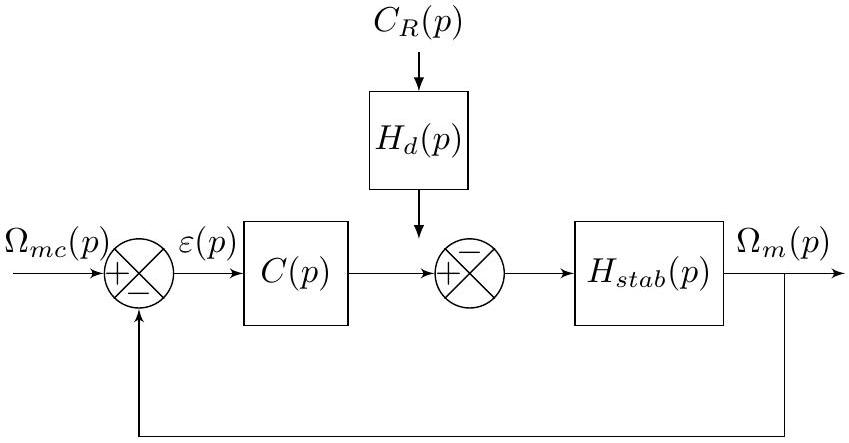
\includegraphics[alt={},max width=\textwidth]{cd8229cf-9637-40cc-9aaf-03c75c002f2c-12_443_849_1025_616}
\captionsetup{labelformat=empty}
\caption{Figure 7 - Schéma-blocs simplifié de l'asservissement de vitesse angulaire de l'actionneur}
\end{center}
\end{figure}

Pour limiter les oscillations du câble, ainsi que les variations de la vitesse dues aux changements de pentes de la consigne de vitesse angulaire $\omega_{m c}(t)$, l'asservissement de vitesse angulaire du rotor de l'actionneur doit respecter les performances du Tableau 5.

\begin{table}[h]
\begin{center}
\begin{tabular}[t]{|l|l|l|}
\hline
Performances & Critères & Niveaux \\
\hline
\multirow[t]{3}{*}{Stabilité} & Dépassement relatif du $k^{\mathrm{e}}$ dépassement pour une entrée de consigne en échelon, noté $D_{k}^{\%}$ & $D_{k}^{\%}=0 \forall k$ \\
\hline
 & Marge de phase, notée $M \varphi$ & $M \varphi=80^{\circ}$ \\
\hline
 & Marge de gain, notée $M G$ & $M G \geqslant 50 \mathrm{~dB}$ \\
\hline
\multirow[t]{2}{*}{Précision} & Erreur en régime permanent sur la vitesse angulaire de l'actionneur, notée $\mu_{v}$, pour une entrée de consigne en échelon & $\mu_{v}=0$ \\
\hline
 & Sensibilité en régime permanent à une perturbation en échelon & Insensible \\
\hline
\end{tabular}
\captionsetup{labelformat=empty}
\caption{Tableau 5 - Cahier des charges de la boucle d'asservissement de vitesse angulaire}
\end{center}
\end{table}

La stabilisation étudiée dans la Partie D-I, et par le choix d'un facteur d'amortissement $\xi_{s} \geqslant 1$, permettent de considérer que la fonction de transfert de la boucle de stabilisation s'écrit :

$$
H_{s t a b}(p)=\frac{1}{(1+1,24 \cdot p) \cdot(1+0,09 \cdot p)} .
$$

Les ingénieurs proposent un choix de correcteur $C(p)$ du type Proportionnel Intégral, de fonction de transfert :

$$
C(p)=K_{i} \cdot \frac{1+T_{i} \cdot p}{T_{i} \cdot p} .
$$

La détermination du paramètre $T_{i}$ est telle qu'il réalise la compensation du pôle dominant de $H_{\text {stab }}(p)$.

\begin{itemize}
  \item[Q26.] Déterminer les deux pôles de $H_{\text {stab }}(p)$. Quel est le pôle dominant et justifier la réponse? En déduire la valeur numérique de $T_{i}$.
\end{itemize}

La Figure 8 fournit le diagramme de Bode de la fonction de transfert en boucle ouverte corrigée pour $K_{i}=1$ et la compensation du pôle dominant.

\begin{figure}[h]
\begin{center}
  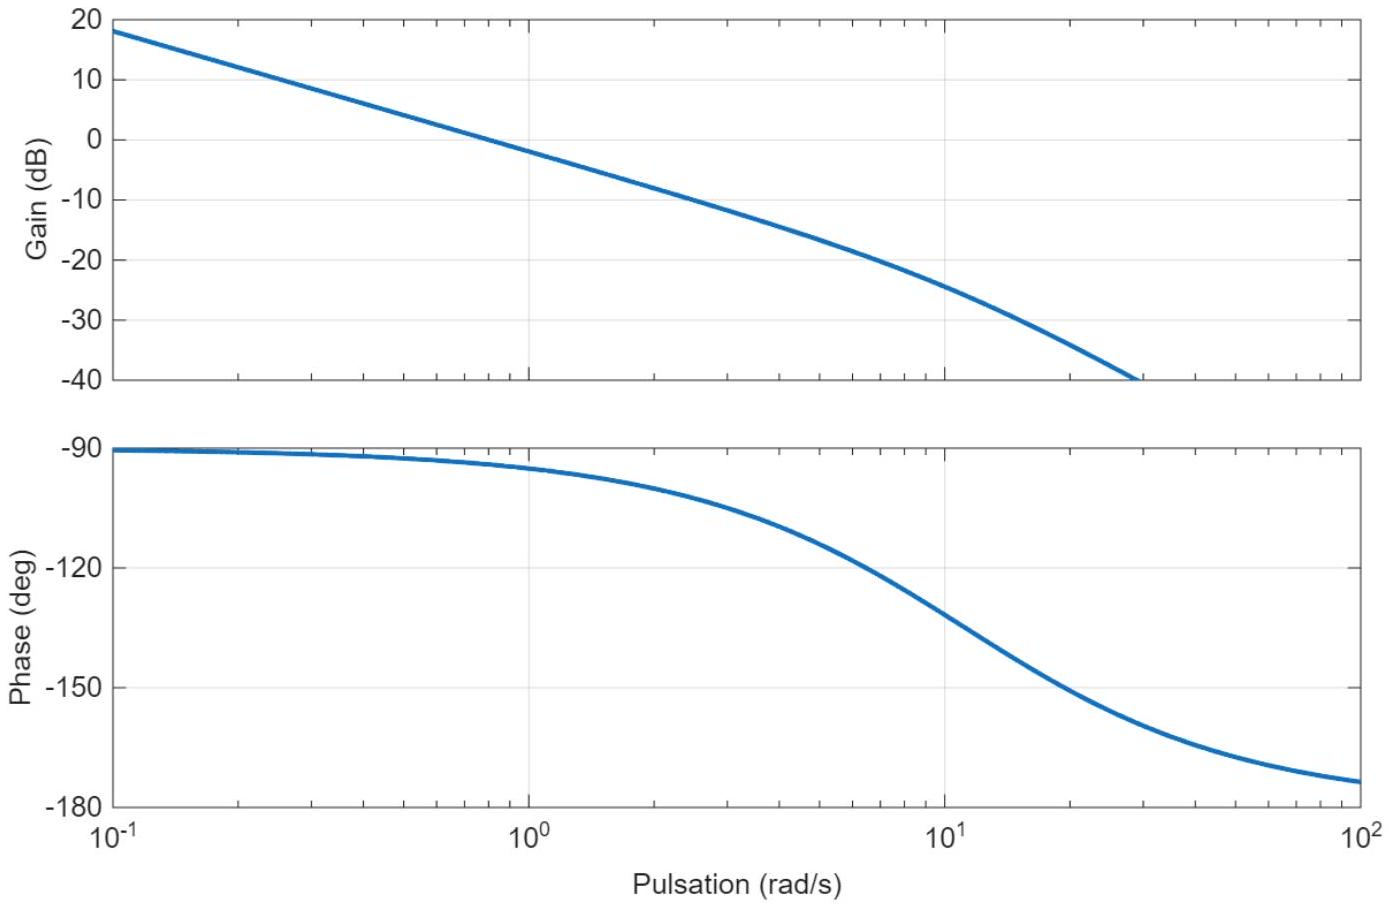
\includegraphics[alt={},max width=\textwidth]{cd8229cf-9637-40cc-9aaf-03c75c002f2c-13_907_1389_377_338}
\captionsetup{labelformat=empty}
\caption{Figure 8 - Diagramme de Bode de la fonction de transfert en boucle ouverte corrigée pour $K_{i}=1$ et compensation du pôle dominant}
\end{center}
\end{figure}

\begin{itemize}
  \item[Q27.] Déterminer numériquement la condition sur le paramètre $K_{i}$ permettant de satisfaire simultanément les critères de stabilité relatifs aux marges de gain et de phase.
\end{itemize}

Par calculs ou par manipulations du schéma-blocs de la Figure 7, il est possible de démontrer que la fonction de transfert $G(p)=\frac{\Omega_{m}(p)}{C_{R}(p)}$ s'écrit sous la forme :

$$
G(p)=\frac{\Omega_{m}(p)}{C_{R}(p)}=\frac{a_{0} \cdot p^{2}}{b_{0}+b_{1} \cdot p+b_{2} \cdot p^{2}+b_{3} \cdot p^{3}} .
$$

Soit $n$ le nombre de passagers embarqués dans la nacelle. Considérons $c_{R}(t)=C_{R 0}(n)=$ constante.

\begin{itemize}
  \item[Q28.] Montrer que, quelque soit $n$, la masse de $n$ passagers dans la nacelle n'a pas d'influence sur la vitesse et la position de la nacelle en régime permanent.
\end{itemize}

La Figure 9 fournit le diagramme de Bode de la fonction de transfert en boucle fermée $F T B F(p)=\frac{\Omega_{m}(p)}{\Omega_{m c}(p)}$ et pour les valeurs pertinentes des paramètres du correcteur $C(p)$.

\begin{itemize}
  \item[Q29.] Conclure quant à la satisfaction ou non de l'intégralité des performances attendues du cahier des charges du Tableau 5.
\end{itemize}

Les études précédentes ont permis de déterminer une modélisation de la commande de l'actionneur afin de contrôler les grandeurs cinématiques. Il est donc désormais possible de vérifier les exigences liées à la sécurité, au panorama et au confort des passagers pour le cycle de vitesse souhaité décrit en partie A-I.

\begin{figure}[h]
\begin{center}
  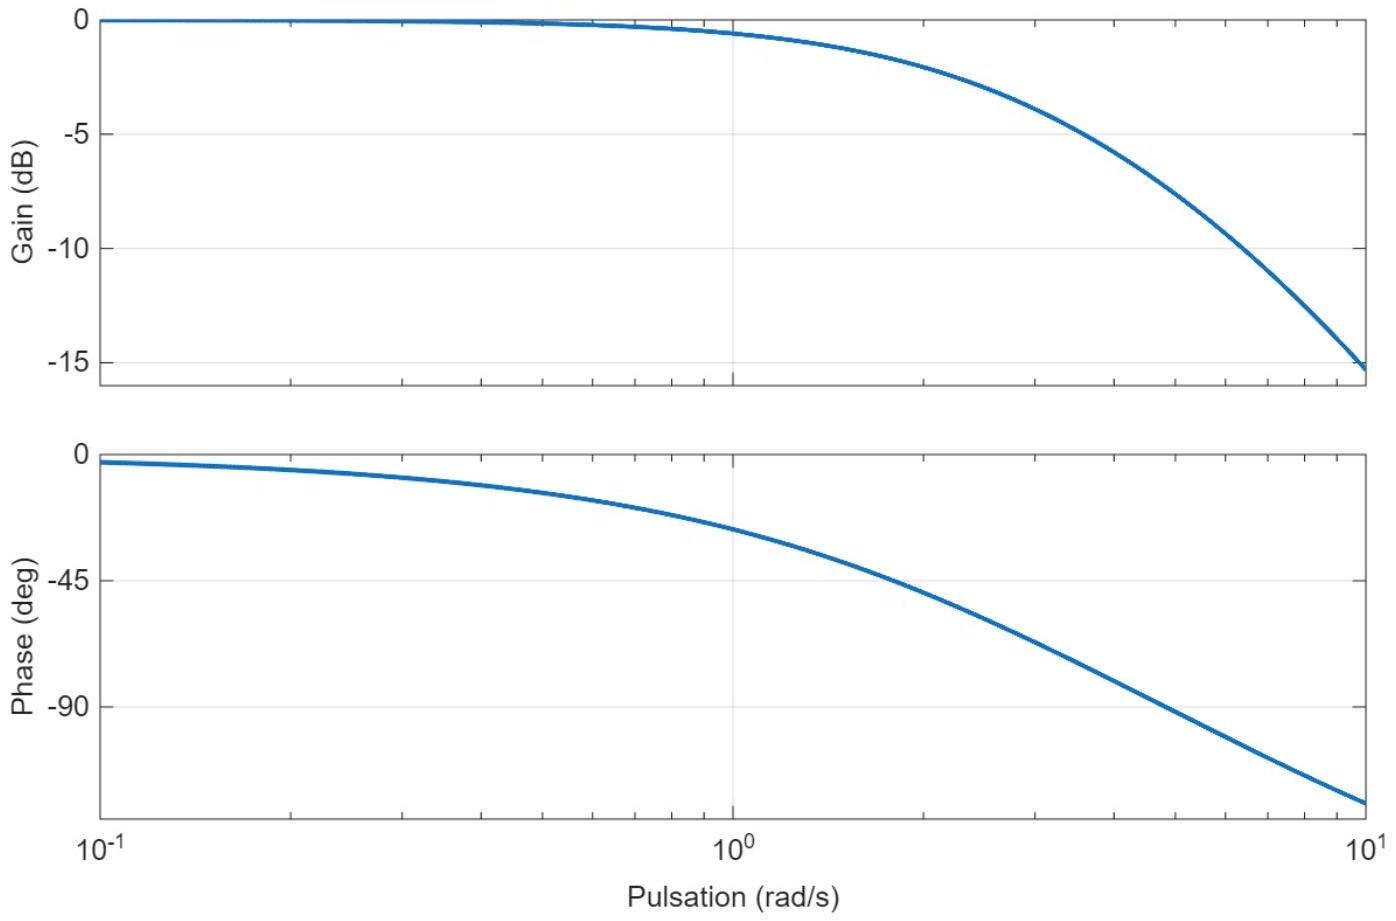
\includegraphics[alt={},max width=\textwidth]{cd8229cf-9637-40cc-9aaf-03c75c002f2c-14_921_1396_121_336}
\captionsetup{labelformat=empty}
\caption{Figure 9 - Diagramme de Bode de $F T B F(p)$}
\end{center}
\end{figure}

\section*{III - Vérification des performances liées à la sécurité et au confort des passagers}
Objectif\\
Caractériser les écarts entre les performances attendues liées à la sécurité et au confort des passagers et les performances simulées (hors critères d'accessibilité de la nacelle et de panorama définis Partie A-I).

L'ensemble des paramètres du modèle de la Figure 4 et les grandeurs d'entrées sont à présents connus. On considère le cycle ascensionnel de vitesse souhaitée de la nacelle $N$ établi en partie A-I, en absence de passager $n=0$ et en présence de $n=200$ passagers dans la nacelle.

Un frein mécanique permet de maintenir à l'arrêt la nacelle (en $z=0 \mathrm{~m}$ et à l'altitude maximale). On considère qu'à l'instant $t=0$ de la simulation, l'actionneur délivre un couple $c_{\text {em }}(t)$ tel que $c_{\text {em }}(t=0)=C_{R 0}(n)$ où $n$ représente le nombre de passagers embarqués dans la nacelle.\\
La simulation du modèle établi dans ce sujet permet d'obtenir les Figures 10 et 11 qui décrivent les évolutions des grandeurs cinématiques de la nacelle $N$.

\begin{figure}[h]
\begin{center}
  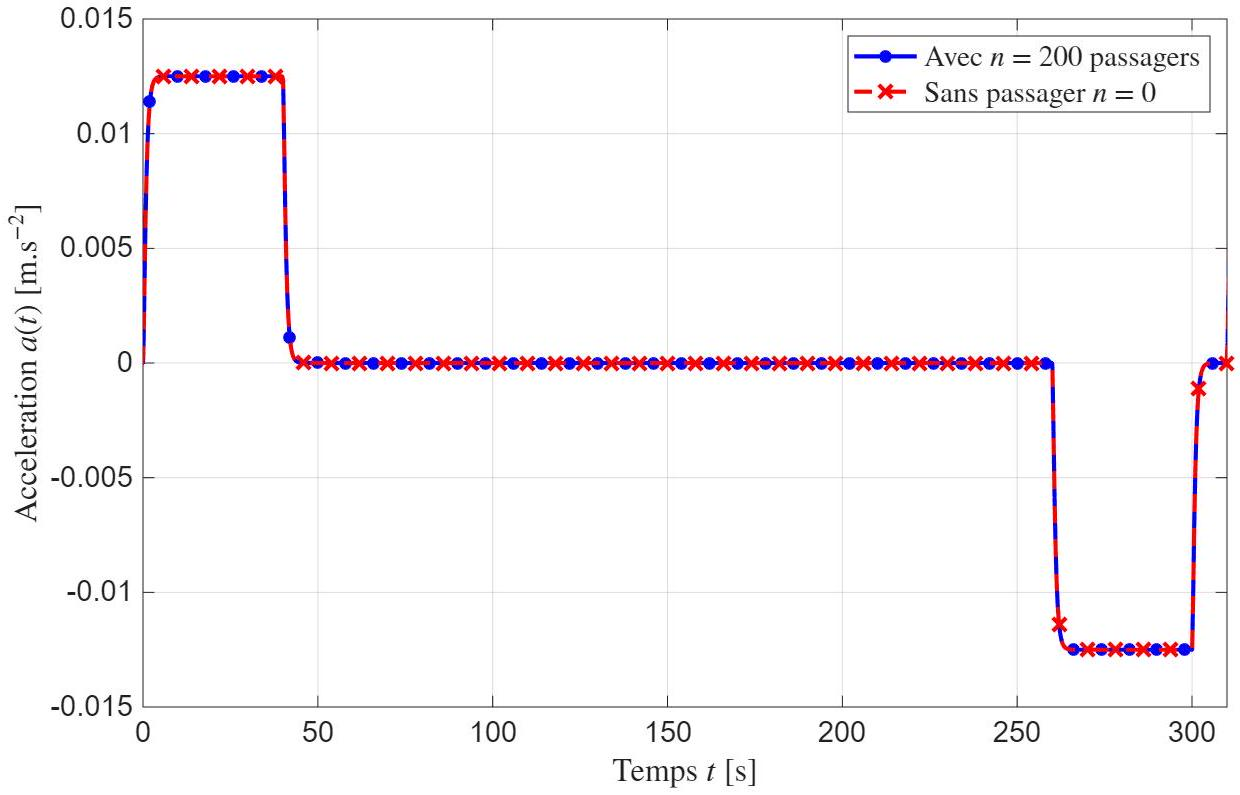
\includegraphics[alt={},max width=\textwidth]{cd8229cf-9637-40cc-9aaf-03c75c002f2c-14_795_1240_1864_413}
\captionsetup{labelformat=empty}
\caption{Figure 10 - Évolution des accélérations linéaires de la nacelle en fonction du nombre de passagers $n$}
\end{center}
\end{figure}

\begin{figure}[h]
\begin{center}
  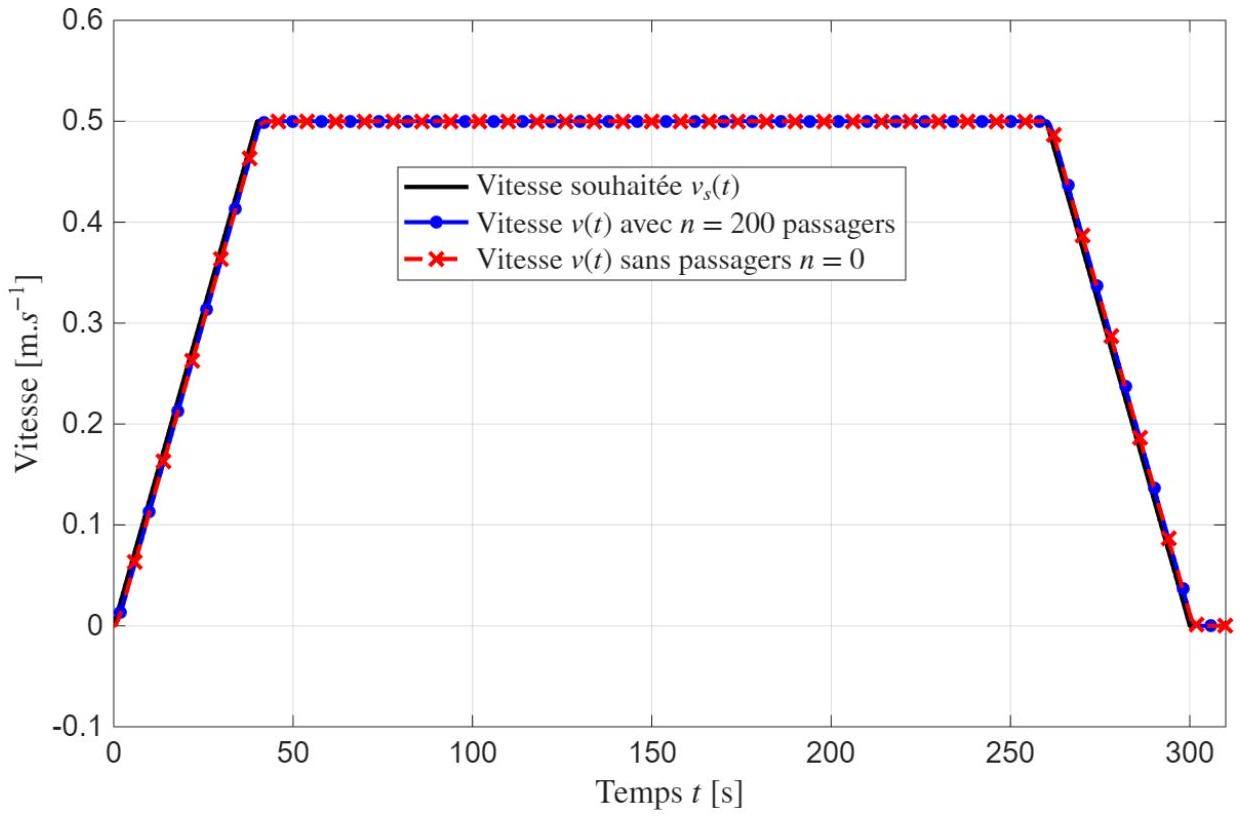
\includegraphics[alt={},max width=\textwidth]{cd8229cf-9637-40cc-9aaf-03c75c002f2c-15_816_1240_121_413}
\captionsetup{labelformat=empty}
\caption{Figure 11 - Évolution des vitesses linéaires de la nacelle en fonction du nombre de passagers $n$}
\end{center}
\end{figure}

Q30. Conclure quant à la satisfaction ou non des critères des exigences liées à la sécurité et au confort des passagers (Tableau 2), quelque soit le nombre de passagers embarqués dans la nacelle $N$.

\section*{Partie E - Vérification de l'exigence liée à la consommation d'énergie et analyse d'une évolution structurelle de l'ouvrage}
Objectif\\
Vérifier l'exigence de consommation d'énergie électrique imposée par le commanditaire et analyser l'influence d'une évolution structurelle de l'ouvrage sur la consommation énergétique électrique de l'actionneur.

Le modèle établi dans ce sujet permet d'évaluer, par simulation, les énergies mises en jeu sur un cycle ascensionnel et descensionnel de la nacelle tel que défini dans la Partie A-I.\\
Hypothèses

\begin{itemize}
  \item[-] les hypothèses formulées dans les parties précédentes sont maintenues (sauf celle remise en cause en Partie C-III) ;
  \item[-] seules les pertes par effet Joule dans l'actionneur sont prises en compte (pertes Fer, pertes par hystérésis... négligées).
\end{itemize}

Notations

\begin{itemize}
  \item[-] la puissance dissipée par effet Joule dans l'actionneur, notée $p_{J}(t)$, est définie par $p_{J}(t)=R_{s} \cdot\left(i_{d s}^{2}(t)+i_{q s}^{2}(t)\right)$. Les grandeurs $i_{d s}(t)$ et $i_{q s}(t)$ sont les courants électriques circulant dans l'actionneur. Le paramètre $R_{s}$ est la résistance électrique du stator de l'actionneur ;
  \item[-] la puissance électromagnétique développée par l'actionneur, notée $p_{e m}(t)$, est définie par $p_{e m}(t)=c_{e m}(t) \cdot \omega_{m}(t)$. Cette grandeur est algébrique. On associe une valeur positive à $p_{e m}(t)$ lorsque l'actionneur fonctionne en mode moteur et que la conversion de puissance est réalisée dans le sens électrique vers mécanique. De même, on associe une valeur négative à $p_{e m}(t)$ lorsque l'actionneur fonctionne en mode générateur et que la conversion de puissance est réalisée dans le sens mécanique vers électrique (l'énergie est renvoyée sur le réseau d'alimentation via le préactionneur) ;
  \item[-] l'énergie mécanique fournie par l'actionneur, notée $E_{m}(t)$, définie par $E_{m}(t)=\int_{t_{0}=0}^{t} p_{e m}(x) \cdot \mathrm{d} x$;
  \item[-] l'énergie dissipée par effet Joule dans l'actionneur, notée $E_{J}(t)$, définie par $E_{J}(t)=\int_{t_{0}=0}^{t} p_{J}(x) \cdot \mathrm{d} x$;
  \item[-] l'énergie électrique consommée par l'actionneur, notée $E_{e}(t)$, définie par $E_{e}(t)=E_{m}(t)+E_{J}(t)$.
\end{itemize}

La simulation du modèle établi, dans les cas sans passager $(n=0)$ et avec $n=200$ passagers à bord de la nacelle, permet d'obtenir la Figure 12, décrivant les évolutions des énergies mises en jeu pour la mise en mouvement de la nacelle, respectivement pour l'énergie mécanique $E_{m}(t)$ fournie par l'actionneur et l'énergie dissipée par effet Joule dans l'actionneur $E_{J}(t)$.

\begin{figure}[h]
\begin{center}
  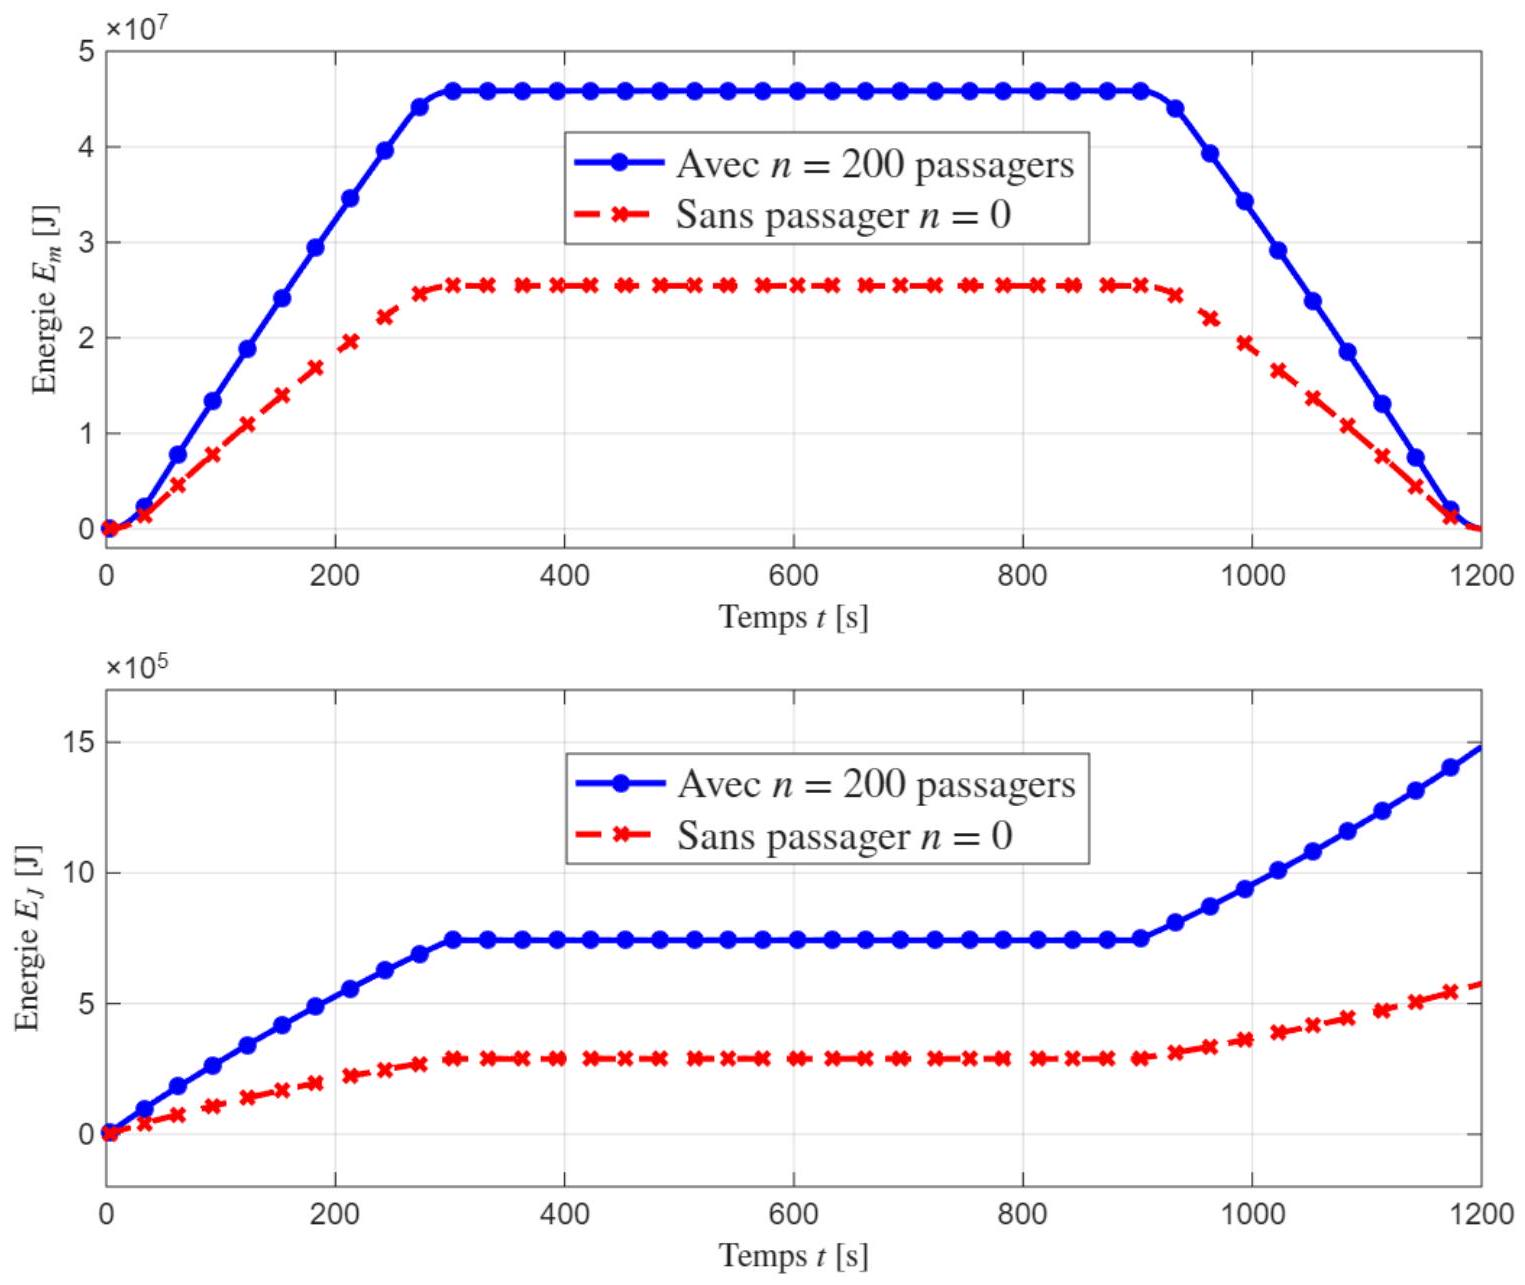
\includegraphics[alt={},max width=\textwidth]{cd8229cf-9637-40cc-9aaf-03c75c002f2c-16_1285_1525_320_269}
\captionsetup{labelformat=empty}
\caption{Figure 12 - Évolutions des énergies $E_{m}(t)$ et $E_{J}(t)$ sur un cycle complet de la nacelle $N$}
\end{center}
\end{figure}

\begin{itemize}
  \item[Q31.] Dans le cas de la présence de $n=200$ passagers à bord de la nacelle, et compte-tenu des hypothèses formulées pour l'obtention du modèle, commenter la valeur numérique de $E_{m}(t=1200 \mathrm{~s})$. Quelles hypothèses (au moins 2) faudrait-il remettre en cause pour obtenir une modélisation plus réaliste ?
\end{itemize}

La structure de l'alimentation de l'actionneur équipant la tour British Airways i360 est proposée sur la Figure 13.

\begin{figure}[h]
\begin{center}
  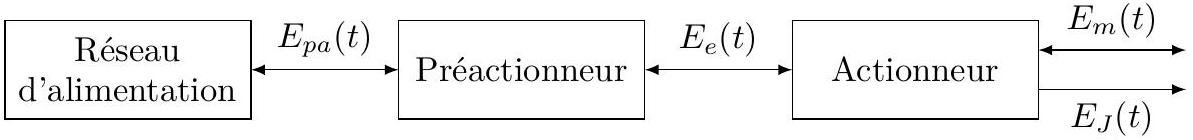
\includegraphics[alt={},max width=\textwidth]{cd8229cf-9637-40cc-9aaf-03c75c002f2c-16_140_1193_1973_438}
\captionsetup{labelformat=empty}
\caption{Figure 13 - Structure fonctionnelle de l'alimentation de l'actionneur}
\end{center}
\end{figure}

Comme tout système, le préactionneur n'est pas idéal énergétiquement, et génère des pertes. De plus, le rendement de ce préactionneur dépend du sens de transfert de l'énergie. En effet, ce préactionneur possède les propriétés suivantes :

\begin{itemize}
  \item[]
  \begin{itemize}
    \item[-] dans le cas d'un fonctionnement moteur de l'actionneur (sens de transfert du domaine électrique vers domaine mécanique, donc $p_{e m}(t)>0$ ), le rendement $\eta_{e \rightarrow m}$ (supposé constant) est défini par $\eta_{e \rightarrow m}=\frac{E_{e}}{E_{p a}}=0,93=93 \%$;
    \item[-] dans le cas d'un fonctionnement générateur de l'actionneur (sens de transfert du domaine mécanique vers domaine électrique, donc $p_{e m}(t)<0$ ), le rendement $\eta_{m \rightarrow e}$ (supposé constant) est défini par $\eta_{m \rightarrow e}=\frac{E_{p a}}{E_{e}}=0,6$ $=60 \%$.
  \end{itemize}
  \item[Q32.] À partir de la Figure 12, et dans le cas de la présence de $n=200$ passagers à bord de la nacelle, déterminer numériquement l'énergie fournie par le réseau d'alimentation pour le cycle ascensionnel de la nacelle, notée
\end{itemize}

$E_{p a, a}=E_{p a}\left(t=t_{3}\right)-E_{p a}\left(t=t_{0}\right)$. De même, déterminer numériquement l'énergie fournie par le réseau d'alimentation pour le cycle descensionnel de la nacelle, notée $E_{p a, d}=E_{p a}\left(t=t_{7}\right)-E_{p a}\left(t=t_{4}\right)<0$. Conclure quant au respect ou non de l'exigence du commanditaire relative à la consommation d'énergie électrique (Tableau 1) à partir du modèle établi dans ce sujet.

Les ingénieurs de la société POMA ont proposé une évolution structurelle dans l'objectif d'améliorer les performances énergétiques de l'ouvrage de la tour British Airways i360. L'embarquement des passagers dans la nacelle $N$ se situe à une altitude $z=4 \mathrm{~m}$ par rapport au sol 0 et le débarquement se situe au niveau du sol $z=0 \mathrm{~m}$. La distance à parcourir en phase ascensionnelle est donc de 126 m , et la distance à parcourir en phase descensionnelle de la nacelle de 130 m. Après débarquement des passagers, la nacelle remonte sans passager d'une hauteur de 4 m.

Q33. Quantifier le gain en \% d'économie d'énergie électrique obtenu par la mise en place de cette évolution structurelle. Les hypothèses simplificatrices doivent être clairement précisées et sont laissées à l'initiative du candidat. Conclure quant à la pertinence de la mise en place de cette évolution structurelle.\\
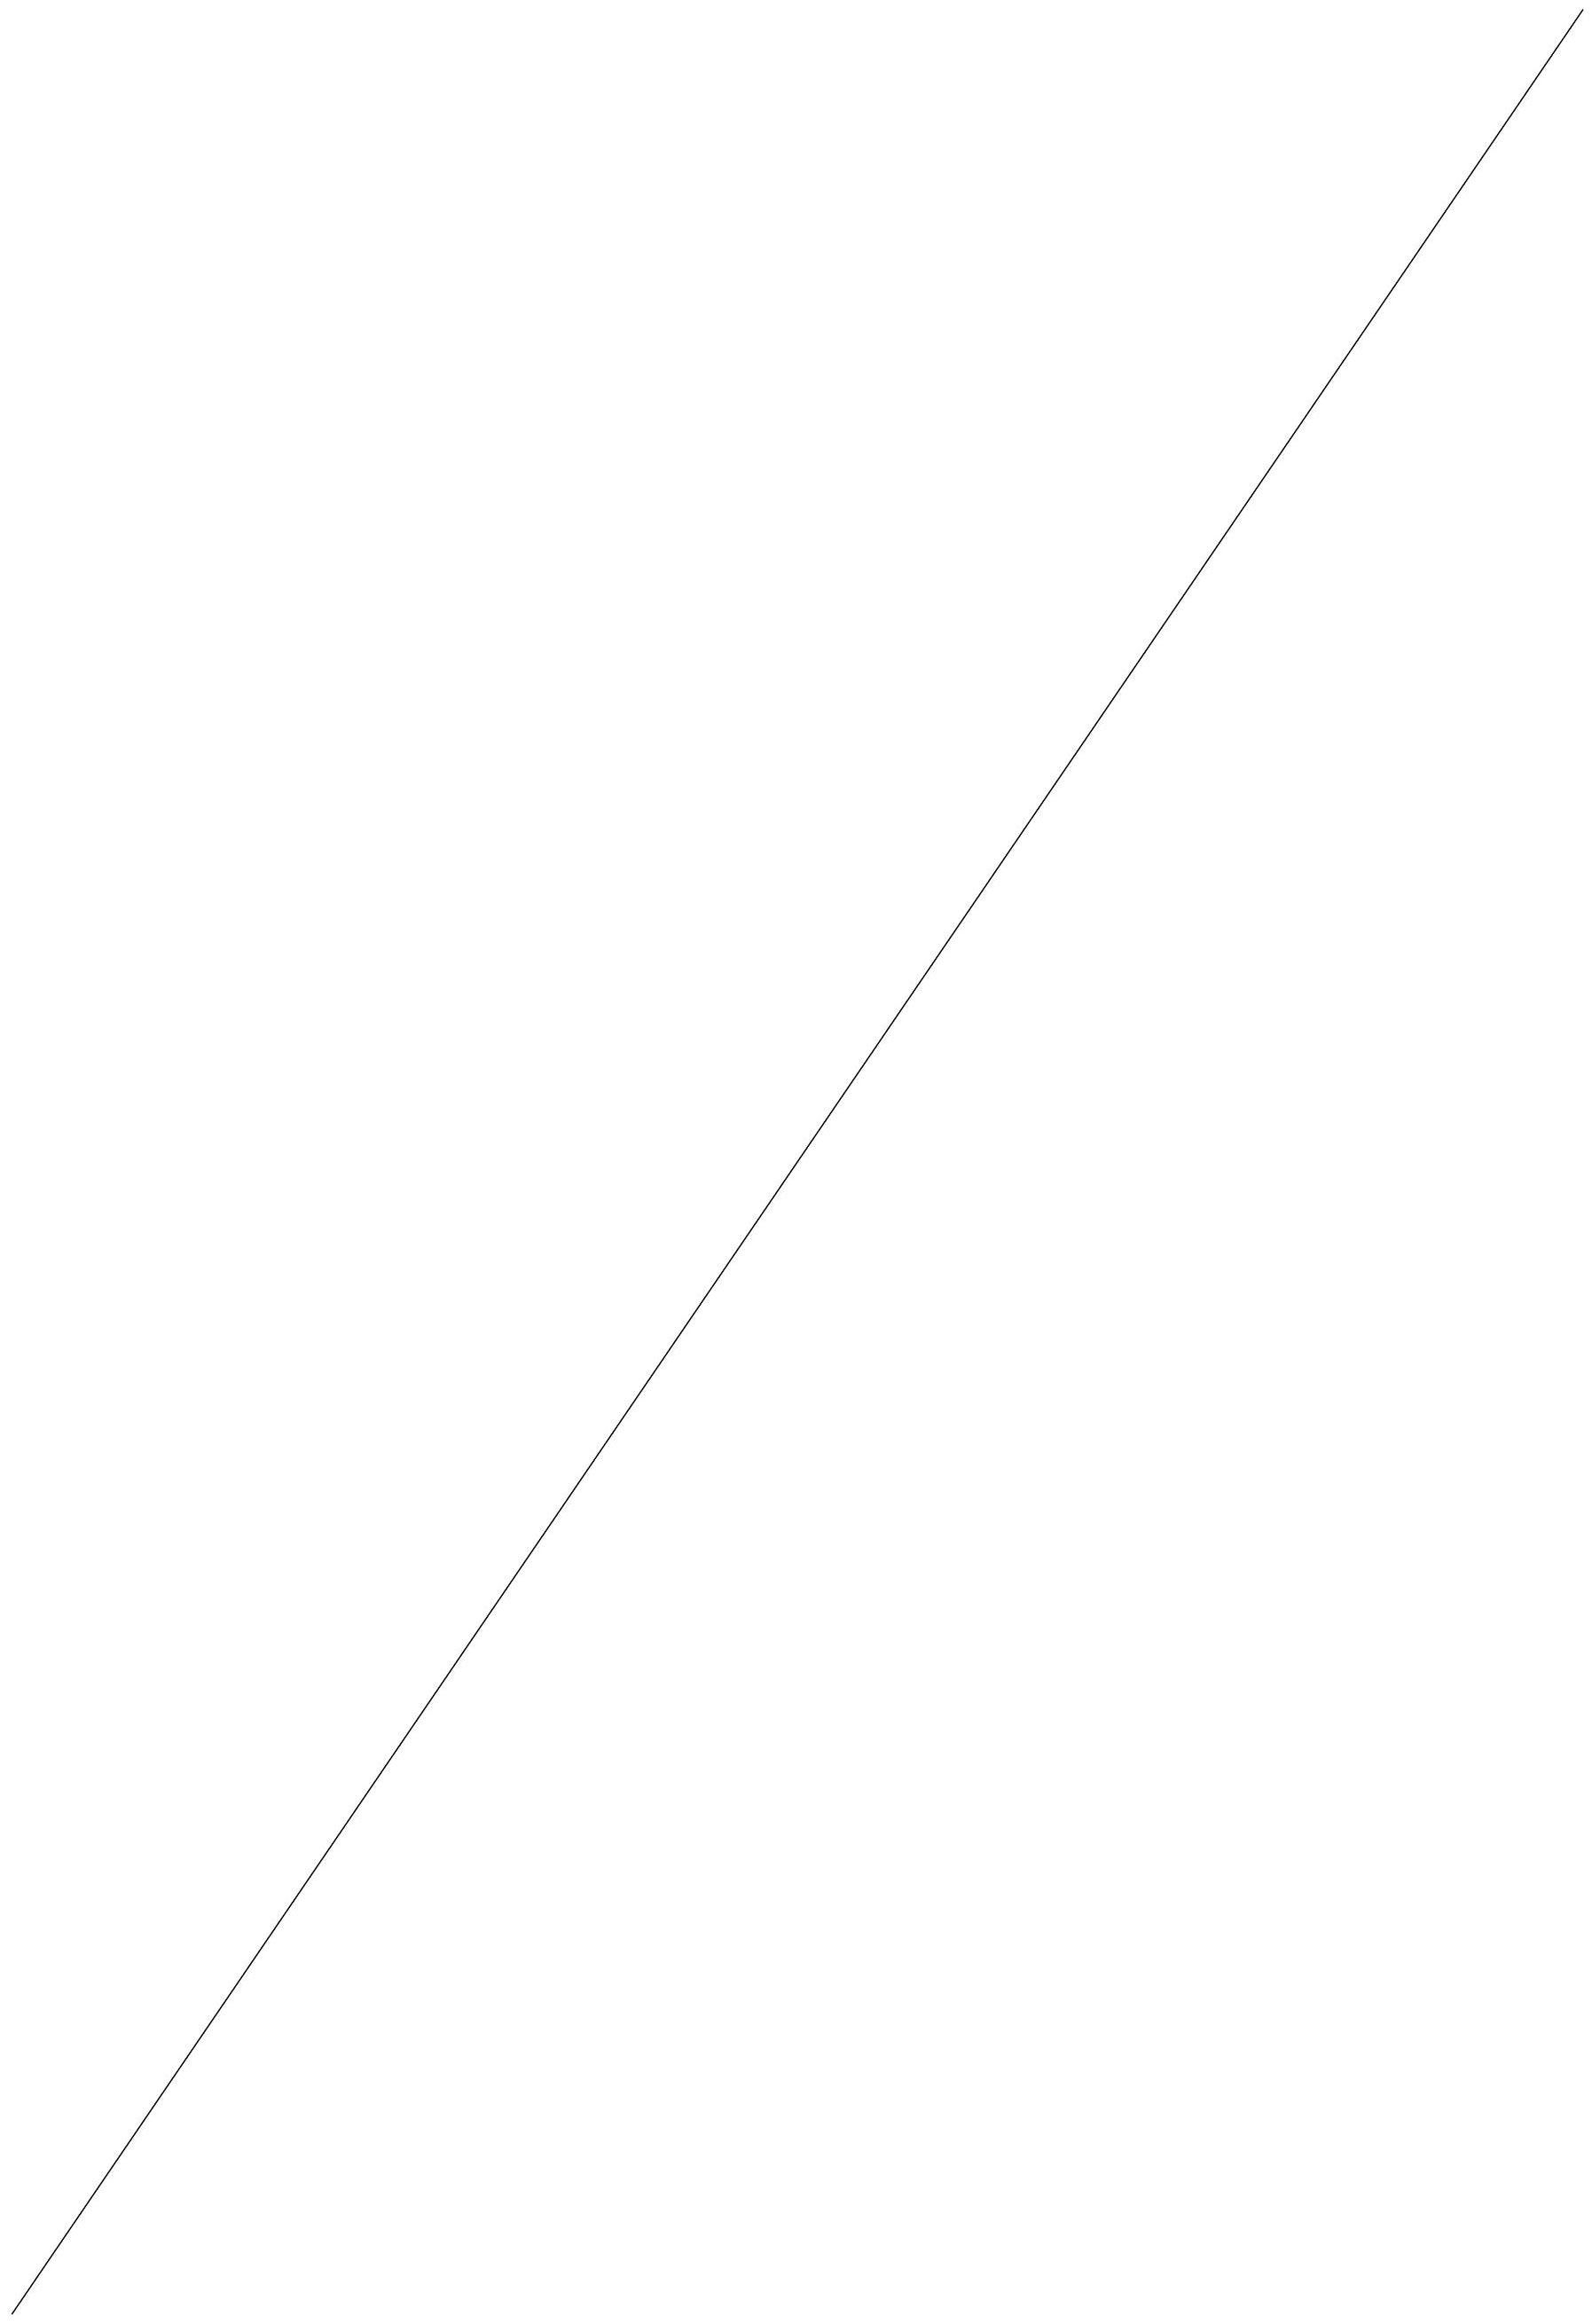
\includegraphics[max width=\textwidth, alt={}, center]{cd8229cf-9637-40cc-9aaf-03c75c002f2c-18_2620_1795_118_135}


\end{document}